% -------------------- Result and Analysis ----------------------------------



\section{Test Plans, Results and Analysis}
%Prepare the test plans in tabular format, where each Test Case should be represented with distinct id, prefixed with “$\langle$module$\rangle$ “, where module represents the short code of the respective design module. Test Case numbers should be matching as stated in Requirement Matrix.
%\vspace{.1in}

%\noindent

%Appropriate definition of ‘Performance Metrics’, e.g. Classification Accuracy, Mean Squared Error etc. should be included, as applicable. 
%\vspace{.1in}

%\noindent
%Depending on your specific project, test results can be represented as a table of data with a corresponding pie chart / bar chart as needed. Analysis of test results should be discussed in terms of clear bullet points.
\begin{center}
    \textbf{Test Case Plan Table}
\end{center}

\begin{table}[h!]
    \centering
    \resizebox{\textwidth}{!}{
    \begin{tabularx}{\textwidth}{|>{\centering\arraybackslash}m{1.5cm}|X|X|X|>{\centering\arraybackslash}m{1.5cm}|}
        \hline
        \textbf{Test Case ID} & \textbf{Description} & \textbf{Expected Result} & \textbf{Actual Result} & \textbf{Status} \\ \hline
        T01 & User provides input in the text area. & Text is accepted for further processing. & Text is accepted for further processing. & \checkmark \\ \hline
        T02 & Display mental health issues with probabilities for classes. & Probabilities for each mental health class are shown. & Probabilities for each mental health class are shown. & \checkmark \\ \hline
        T03 & Highlight the mental health issue with the highest probability. & Correct issue with the highest probability is displayed. & Correct issue with the highest probability is displayed. & \checkmark \\ \hline
        T04 & Accept username input and provide prediction. & Prediction is displayed based on the provided username. & Prediction is displayed based on the provided username. & \checkmark \\ \hline
        T05 & Translate multiple language inputs to English. & Non-English text is translated correctly to English. & Non-English text is translated correctly to English. & \checkmark \\ \hline
        T06 & Extract text and detect emotion from image. & Extracted text and detected emotions are displayed accurately. & Extracted text and detected emotions are displayed accurately. & \checkmark \\ \hline
        T07 & Pass a prompt to the system and retrieve a valid response. & Correct response is generated based on the prompt. & Correct response is generated based on the prompt. & \checkmark \\ \hline
        T08 & Perform a combined test using multiple inputs. & Predictions for all inputs are displayed correctly. & Predictions for all inputs are displayed correctly. & \checkmark \\ \hline
        T09 & Analyze uploaded audio files and transcribe them into text. & Audio transcription and analysis results are displayed. & Audio transcription and analysis results are displayed. & \checkmark \\ \hline
        T10 & Extract frames, analyze emotions, audio from video. & Frame emotions and audio transcription are displayed. & Frame emotions and audio transcription are displayed. & \checkmark \\ \hline
        T11 & Extract tweets and related media using a Twitter username. & Text and media are extracted and analyzed correctly. & Text and media are extracted and analyzed correctly. & \checkmark \\ \hline
        T12 & Generate captions for uploaded images or video frames. & Captions are generated for images or frames. & Captions are generated for images or frames. & \checkmark \\ \hline
    \end{tabularx}
    }
    \end{table}

\pagebreak

\noindent
The metrics used for evaluating the performance of the classification models include Precision, Recall, F1-Score, and Support, along with the Confusion Matrix. These metrics are crucial for assessing how well the models are able to differentiate between various classes, providing insight into their accuracy, ability to capture relevant instances, and the overall balance between precision and recall. By analyzing these metrics, a comprehensive understanding of the model's performance can be obtained, enabling informed decisions for further optimization and tuning.

\subsection{Classification Metrics and Confusion Matrix}

\begin{itemize}
    \item \textbf{Precision:} Precision is the ratio of correctly predicted positive observations to the total predicted positives. It can be calculated as:
    \[
    \text{Precision} = \frac{TP}{TP + FP}
    \]
    where \( TP \) represents True Positives, and \( FP \) represents False Positives.

    \item \textbf{Recall:} Recall is the ratio of correctly predicted positive observations to all observations in the actual class:
    \[
    \text{Recall} = \frac{TP}{TP + FN}
    \]
    where \( TP \) is True Positives, and \( FN \) is False Negatives.

    \item \textbf{F1-Score:} F1-Score is the harmonic mean of Precision and Recall, calculated as:
    \[
    \text{F1-Score} = 2 \times \frac{\text{Precision} \times \text{Recall}}{\text{Precision} + \text{Recall}}
    \]

    \item \textbf{Support:} Support refers to the number of actual occurrences of each class in the dataset:
    \[
    \text{Support} = \text{Number of samples in the true class}
    \]

    \item \textbf{Confusion Matrix:} A confusion matrix is used to evaluate the performance of a classification model. It is structured as follows:
    \[
    \begin{bmatrix}
    TP & FP \\
    FN & TN
    \end{bmatrix}
    \]
    where:
    \begin{itemize}
        \item \( TP \) = True Positives
        \item \( FP \) = False Positives
        \item \( FN \) = False Negatives
        \item \( TN \) = True Negatives
    \end{itemize}
\end{itemize}

\subsection{Results of Logistic Regression}

\begin{center}
    \textbf{Logistic Regression Classification Report} \\[0.5em]
    \begin{tabular}{|l|c|c|c|c|}
        \hline
        \textbf{Class} & \textbf{Precision} & \textbf{Recall} & \textbf{F1-Score} & \textbf{Support} \\ \hline
        Anxiety        & 0.83               & 0.77            & 0.80              & 379              \\ \hline
        Bipolar        & 0.74               & 0.55            & 0.63              & 384              \\ \hline
        Depression     & 0.76               & 0.76            & 0.76              & 373              \\ \hline
        Normal         & 0.92               & 0.99            & 0.95              & 2183             \\ \hline
        PTSD           & 0.87               & 0.77            & 0.82              & 394              \\ \hline
        \textbf{Accuracy} & \multicolumn{4}{|c|}{87.66\%} \\ \hline
        \textbf{Macro Avg} & 0.82            & 0.77            & 0.79              & 3713             \\ \hline
        \textbf{Weighted Avg} & 0.87         & 0.88            & 0.87              & 3713             \\ \hline
    \end{tabular}
\end{center}

\vspace{0.25em}

\begin{center}
    \textbf{ROC Curve Areas for Each Class} \\[0.5em]
    \begin{tabular}{|l|c|}
        \hline
        \textbf{Class}  & \textbf{ROC AUC} \\ \hline
        Anxiety         & 0.95            \\ \hline
        Bipolar         & 0.92            \\ \hline
        Depression      & 0.96            \\ \hline
        Normal          & 0.99            \\ \hline
        PTSD            & 0.95            \\ \hline
    \end{tabular}
\end{center}

\vspace{0.25em}

\begin{figure}[h!]  
    \centering
    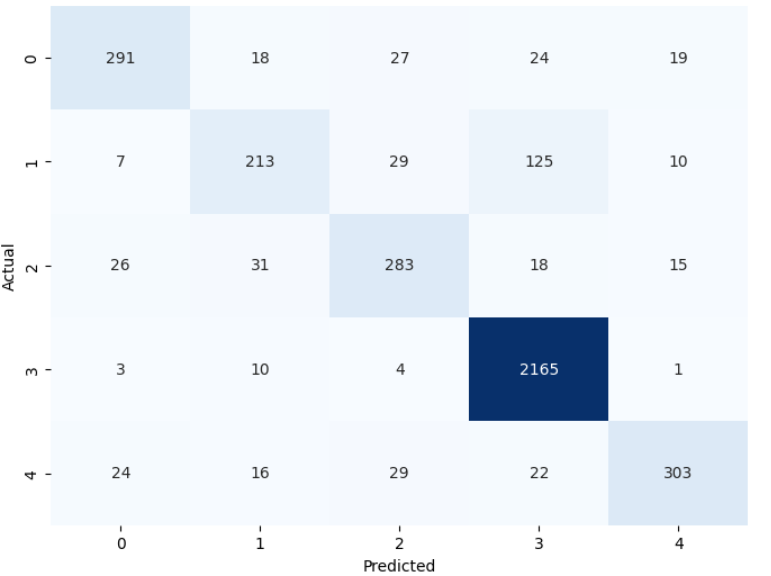
\includegraphics[width=0.7\textwidth]{Images/LR Confusion Matrix.png}  
    \caption{Confusion Matrix (Logistic Regression)}
    \label{LRCM}  % Label for referencing the figure
\end{figure}

\begin{figure}[h!]  
    \centering
    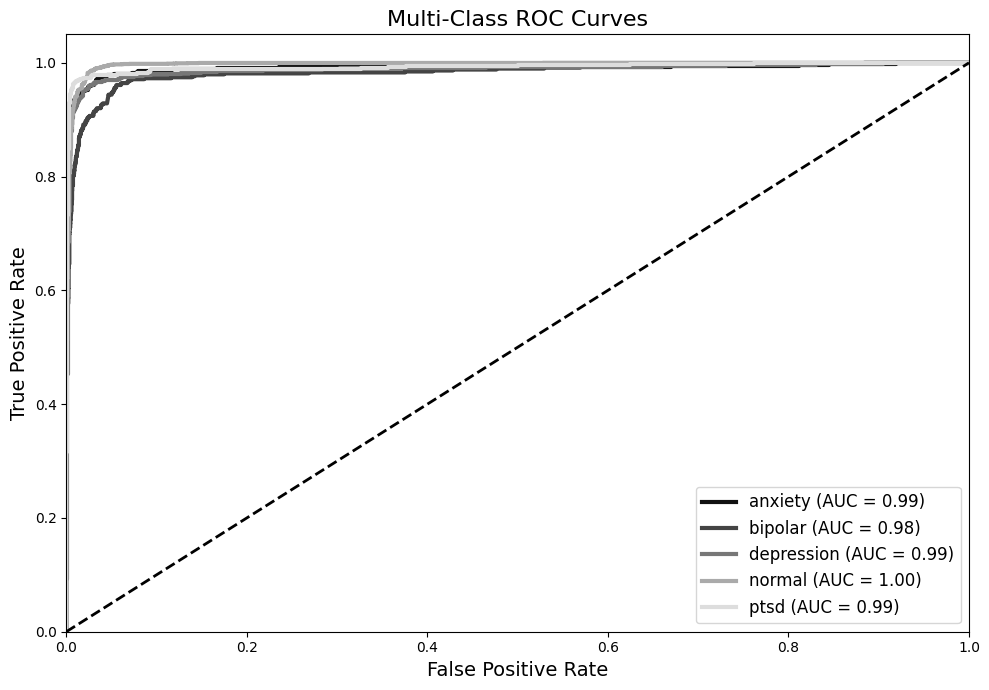
\includegraphics[width=0.7\textwidth]{Images/LR ROC.png}  
    \caption{ROC AUC (Logistic Regression)}
    \label{LRROC}  % Label for referencing the figure
\end{figure}

\noindent
The Logistic Regression model performed well with an overall accuracy of 87.66\%, indicating that the model correctly classified the majority of the instances. The classification report shows high precision, recall, and F1-scores for the 'Normal' class, which was expected due to its large number of instances. However, the 'Bipolar' and 'Anxiety' classes have lower recall and F1-scores, suggesting that the model struggles more with these classes. The confusion matrix highlights the misclassifications. For example, 'Anxiety' is often confused with 'Depression' and 'PTSD,' while the 'Normal' class is well-separated from the other classes. The large number of instances in the 'Normal' class could have contributed to the high accuracy but also to the imbalance in performance across other classes. The ROC curve AUC scores indicate that the model performs well in distinguishing between the classes. The 'Normal' class has the highest AUC (0.99), which is expected due to the large proportion of 'Normal' instances. Other classes, like 'Anxiety' and 'Depression,' also have high AUC scores (0.95 and 0.96, respectively), indicating that the model is capable of distinguishing them effectively.

% --------- naive bayes

\subsection{Results of Naive Bayes}

\begin{center}
    \textbf{Naive Bayes Classification Report} \\[0.5em]
    \begin{tabular}{|l|c|c|c|c|}
        \hline
        \textbf{Class} & \textbf{Precision} & \textbf{Recall} & \textbf{F1-Score} & \textbf{Support} \\ \hline
        Anxiety        & 0.70               & 0.73            & 0.72              & 379              \\ \hline
        Bipolar        & 0.83               & 0.45            & 0.58              & 384              \\ \hline
        Depression     & 0.59               & 0.87            & 0.70              & 373              \\ \hline
        Normal         & 0.96               & 0.92            & 0.94              & 2183             \\ \hline
        PTSD           & 0.71               & 0.83            & 0.76              & 394              \\ \hline
        \textbf{Accuracy} & \multicolumn{4}{|c|}{83.63\%} \\ \hline
        \textbf{Macro Avg} & 0.76            & 0.76            & 0.74              & 3713             \\ \hline
        \textbf{Weighted Avg} & 0.85         & 0.84            & 0.84              & 3713             \\ \hline
    \end{tabular}
\end{center}

\vspace{0.25em}

\begin{center}
    \textbf{ROC Curve Areas for Each Class} \\[0.5em]
    \begin{tabular}{|l|c|}
        \hline
        \textbf{Class}  & \textbf{ROC AUC} \\ \hline
        Anxiety         & 0.92            \\ \hline
        Bipolar         & 0.89            \\ \hline
        Depression      & 0.94            \\ \hline
        Normal          & 0.99            \\ \hline
        PTSD            & 0.94            \\ \hline
    \end{tabular}
\end{center}

\vspace{0.25em}

\begin{figure}[h!]  
    \centering
    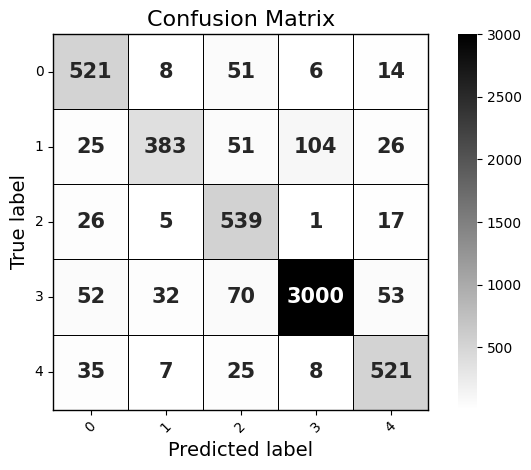
\includegraphics[width=0.7\textwidth]{Images/NB Confusion Matrix.png}  
    \caption{Confusion Matrix (Naive Bayes)}
    \label{NBCM}  % Label for referencing the figure
\end{figure}


\begin{figure}[h!]  
    \centering
    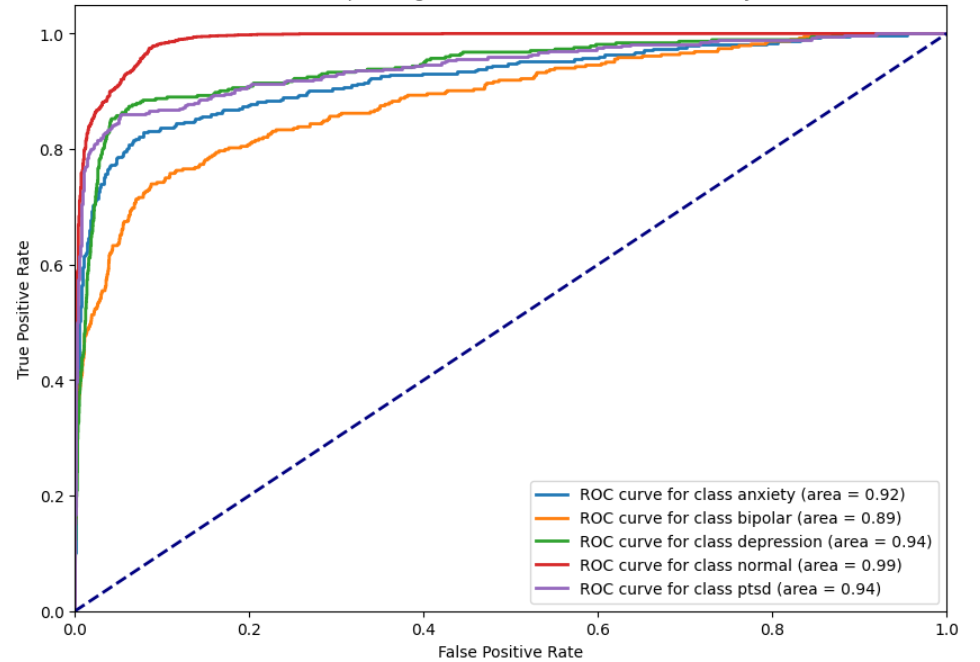
\includegraphics[width=0.7\textwidth]{Images/NB ROC.png}  
    \caption{ROC AUC (Naive Bayes)}
    \label{NBROC}  % Label for referencing the figure
\end{figure}

\noindent
The Naive Bayes model achieved an overall accuracy of 83.63\%, indicating a reasonable performance. The classification report shows strong results for the Normal class, with a precision of 0.96 and a recall of 0.92, resulting in an F1-score of 0.94. However, the Bipolar class exhibits much lower recall (0.45) and F1-score (0.58), suggesting that the model struggles to accurately identify Bipolar instances. Misclassifications are more frequent for Bipolar, often being confused with Depression and PTSD. The Anxiety class, although having decent precision (0.70), shows a lower recall (0.73), indicating that it also faces challenges in classification. The Confusion Matrix highlights that the model has difficulty distinguishing Bipolar and Depression from each other, with a large number of misclassifications across these classes. On the other hand, the Normal class is well-separated and correctly classified, with 2006 true positives, which likely contributes to the high overall accuracy. PTSD also shows relatively good classification results, with misclassifications being less frequent. The ROC AUC Curve Areas show that the model performs well for most classes, with the Normal class having the highest AUC score (0.99), followed by Depression and PTSD with AUCs of 0.94. While the model performs well for distinguishing between classes like Normal and Depression, the lower AUC for Bipolar (0.89) indicates that there may still be room for improvement in distinguishing this class from others.

% ------------- svc

\subsection{Results of Support Vector Machine}

\begin{center}
    \textbf{SVM Classification Report} \\[0.5em]
    \begin{tabular}{|l|c|c|c|c|}
        \hline
        \textbf{Class} & \textbf{Precision} & \textbf{Recall} & \textbf{F1-Score} & \textbf{Support} \\ \hline
        Anxiety        & 0.72               & 0.76            & 0.74              & 379              \\ \hline
        Bipolar        & 0.62               & 0.61            & 0.61              & 384              \\ \hline
        Depression     & 0.74               & 0.71            & 0.72              & 373              \\ \hline
        Normal         & 0.94               & 0.95            & 0.95              & 2183             \\ \hline
        PTSD           & 0.78               & 0.74            & 0.76              & 394              \\ \hline
        \textbf{Accuracy} & \multicolumn{4}{|c|}{85.13\%} \\ \hline
        \textbf{Macro Avg} & 0.76            & 0.75            & 0.76              & 3713             \\ \hline
        \textbf{Weighted Avg} & 0.85         & 0.85            & 0.85              & 3713             \\ \hline
    \end{tabular}
\end{center}

\vspace{0.25em}

\begin{center}
    \textbf{ROC Curve Areas for Each Class} \\[0.5em]
    \begin{tabular}{|l|c|}
        \hline
        \textbf{Class}  & \textbf{ROC AUC} \\ \hline
        Anxiety         & 0.96            \\ \hline
        Bipolar         & 0.90            \\ \hline
        Depression      & 0.96            \\ \hline
        Normal          & 0.98            \\ \hline
        PTSD            & 0.96            \\ \hline
    \end{tabular}
\end{center}

\vspace{0.25em}

\begin{figure}[h!]  
    \centering
    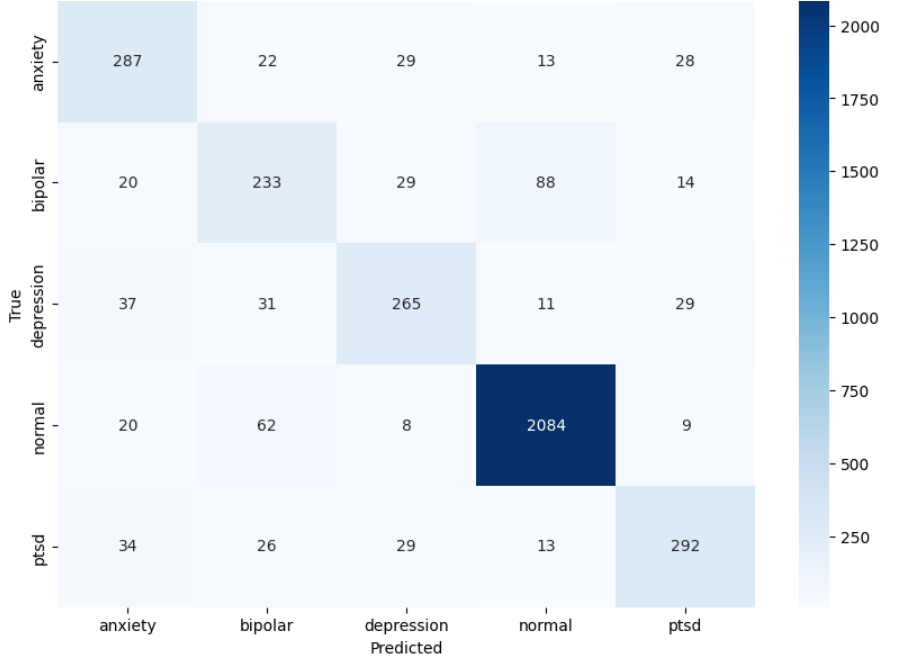
\includegraphics[width=0.7\textwidth]{Images/SVM Confusion Matrix.png}  
    \caption{Confusion Matrix (SVM)}
    \label{SVMCM}  % Label for referencing the figure
\end{figure}

\begin{figure}[h!]  
    \centering
    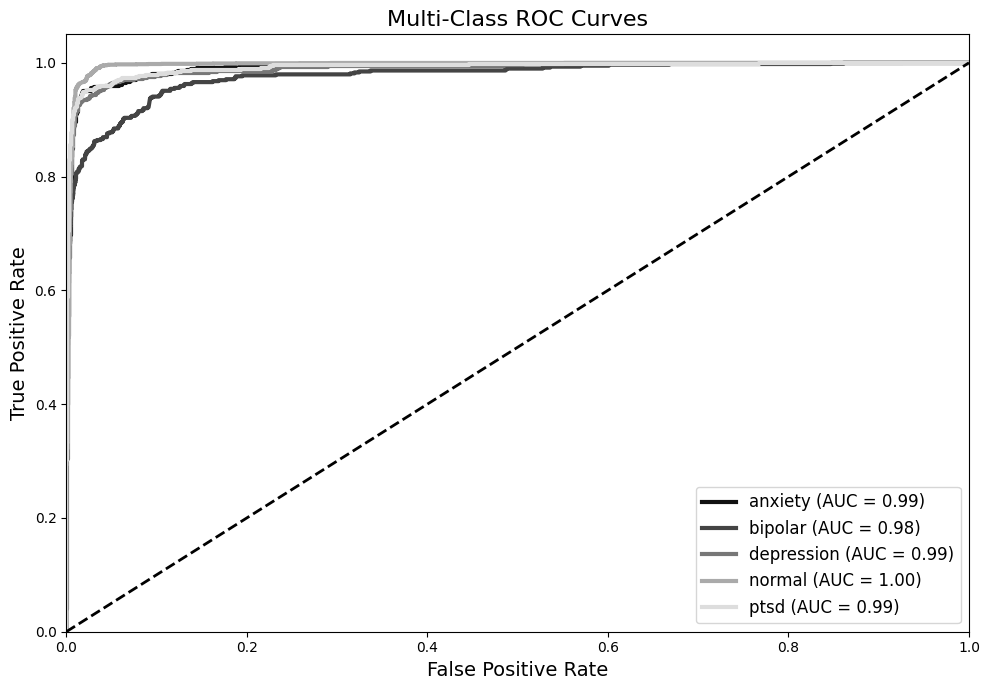
\includegraphics[width=0.7\textwidth]{Images/SVM ROC.png}  
    \caption{ROC AUC (SVM)}
    \label{SVMSOC}  % Label for referencing the figure
\end{figure}

\noindent
The Support Vector Machine (SVM) model achieved an accuracy of 85.13\%, demonstrating strong performance in classifying the various mental health conditions. The classification report indicates that the Normal class has the highest precision (0.94) and recall (0.95), resulting in an F1-score of 0.95, showing that the model is particularly good at identifying instances of normal behavior. However, the Bipolar class shows lower performance, with a precision of 0.62 and recall of 0.61, suggesting that the model struggles more with identifying bipolar disorder instances. The recall for the Anxiety class is relatively high (0.76), though precision is somewhat lower (0.72), indicating a balanced classification performance for this condition. The confusion matrix reveals that the model is generally accurate, with the Normal class being correctly classified most of the time (2084 true positives). However, some misclassifications occur for classes like Bipolar, Depression, and PTSD, with notable misclassifications of Bipolar as Depression and Normal. These misclassifications are likely affecting the overall recall for certain classes. The ROC AUC curve areas demonstrate that the model has excellent performance in distinguishing between most classes. The Normal class has the highest AUC of 0.98, followed by Anxiety, Depression, and PTSD with AUCs of 0.96. Bipolar, although still high at 0.90, lags behind the other classes, reflecting the model's challenge in distinguishing Bipolar from other conditions.

% ------------- random forest

\subsection{Results of Random Forest}

\begin{center}
    \textbf{Random Forest Classification Report} \\[0.5em]
    \begin{tabular}{|l|c|c|c|c|}
        \hline
        \textbf{Class} & \textbf{Precision} & \textbf{Recall} & \textbf{F1-Score} & \textbf{Support} \\ \hline
        Anxiety        & 0.81               & 0.70            & 0.75              & 379              \\ \hline
        Bipolar        & 0.93               & 0.47            & 0.62              & 384              \\ \hline
        Depression     & 0.72               & 0.77            & 0.74              & 373              \\ \hline
        Normal         & 0.88               & 1.00            & 0.93              & 2183             \\ \hline
        PTSD           & 0.92               & 0.74            & 0.82              & 394              \\ \hline
        \textbf{Accuracy} & \multicolumn{4}{|c|}{86.00\%} \\ \hline
        \textbf{Macro Avg} & 0.85            & 0.73            & 0.77              & 3713             \\ \hline
        \textbf{Weighted Avg} & 0.86         & 0.86            & 0.85              & 3713             \\ \hline
    \end{tabular}
\end{center}

\vspace{0.25em}

\begin{center}
    \textbf{ROC Curve Areas for Each Class} \\[0.5em]
    \begin{tabular}{|l|c|}
        \hline
        \textbf{Class}  & \textbf{ROC AUC} \\ \hline
        Anxiety         & 0.96            \\ \hline
        Bipolar         & 0.89            \\ \hline
        Depression      & 0.97            \\ \hline
        Normal          & 0.97            \\ \hline
        PTSD            & 0.97            \\ \hline
    \end{tabular}
\end{center}

\vspace{0.25em}

\begin{figure}[h!]  
    \centering
    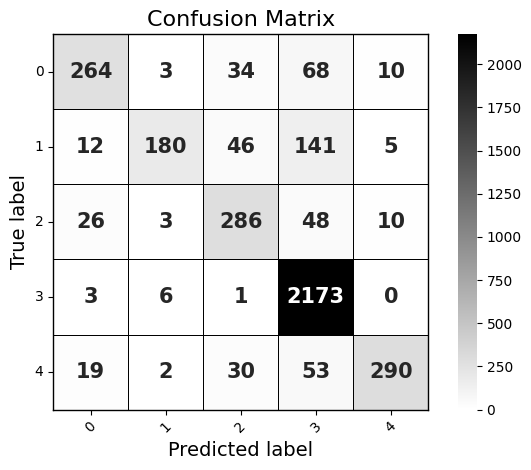
\includegraphics[width=0.7\textwidth]{Images/RF Confusion Matrix.png}  
    \caption{Confusion Matrix (Random Forest)}
    \label{RFCM}  % Label for referencing the figure
\end{figure}

\begin{figure}[h!]  
    \centering
    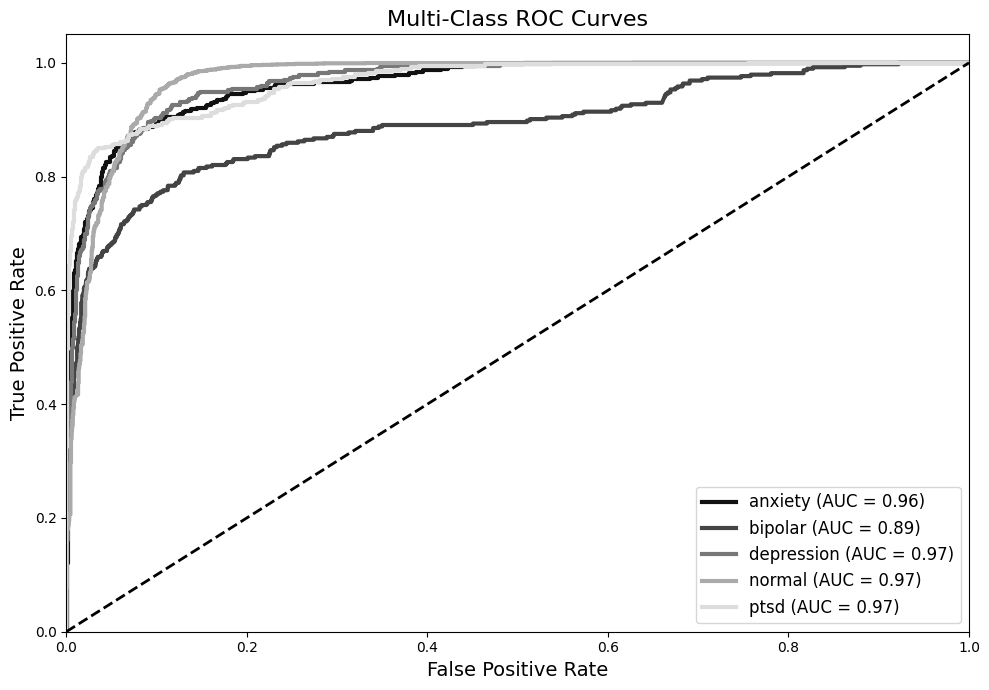
\includegraphics[width=0.7\textwidth]{Images/RF ROC.png}  
    \caption{ROC AUC (Random Forest)}
    \label{RFROC}  % Label for referencing the figure
\end{figure}

\noindent
The Random Forest model achieved an accuracy of 86.00\%, indicating a strong performance in classifying the mental health conditions. The classification report shows that the Normal class achieved the highest recall (1.00) and a precision of 0.88, resulting in a high F1-score of 0.93. This reflects the model’s ability to correctly classify the majority of the Normal instances. The Bipolar class, however, shows a much lower recall (0.47), which indicates that the model has difficulty identifying instances of Bipolar disorder, as reflected by its F1-score of 0.62. The Anxiety and PTSD classes have relatively balanced performance, with moderate precision and recall values. The confusion matrix illustrates the distribution of misclassifications. The Normal class is correctly classified almost entirely (2173 true positives), while other classes like Bipolar and PTSD exhibit significant misclassifications, particularly Bipolar, which is often misclassified as Depression and Normal. The ROC AUC scores for all classes are quite high, indicating that the model is effective at distinguishing between the classes. The Anxiety, Depression, Normal, and PTSD classes each have AUC values above 0.96, with the Normal and Depression classes achieving 0.97. Bipolar has the lowest AUC at 0.89, which corresponds to its lower classification performance. These AUC values suggest that the Random Forest model is proficient in distinguishing between most of the classes, though it faces challenges in identifying Bipolar disorder.

\pagebreak
% -------- xgb

\subsection{Results of XGBoost}

\begin{center}
    \textbf{XGBoost Classification Report} \\[0.5em]
    \begin{tabular}{|l|c|c|c|c|}
        \hline
        \textbf{Class} & \textbf{Precision} & \textbf{Recall} & \textbf{F1-Score} & \textbf{Support} \\ \hline
        Anxiety        & 0.81               & 0.74            & 0.77              & 403              \\ \hline
        Bipolar        & 0.77               & 0.62            & 0.69              & 397              \\ \hline
        Depression     & 0.72               & 0.81            & 0.76              & 387              \\ \hline
        Normal         & 0.93               & 0.98            & 0.95              & 2137             \\ \hline
        PTSD           & 0.86               & 0.75            & 0.80              & 396              \\ \hline
        \textbf{Accuracy} & \multicolumn{4}{|c|}{87.39\%} \\ \hline
        \textbf{Macro Avg} & 0.82            & 0.78            & 0.80              & 3720             \\ \hline
        \textbf{Weighted Avg} & 0.87         & 0.87            & 0.87              & 3720             \\ \hline
    \end{tabular}
\end{center}

\vspace{0.25em}

\begin{center}
    \textbf{ROC Curve Areas for Each Class} \\[0.5em]
    \begin{tabular}{|l|c|}
        \hline
        \textbf{Class}  & \textbf{ROC AUC} \\ \hline
        Anxiety         & 0.97            \\ \hline
        Bipolar         & 0.95            \\ \hline
        Depression      & 0.97            \\ \hline
        Normal          & 0.99            \\ \hline
        PTSD            & 0.97            \\ \hline
    \end{tabular}
\end{center}

\vspace{0.25em}

\begin{figure}[h!]  
    \centering
    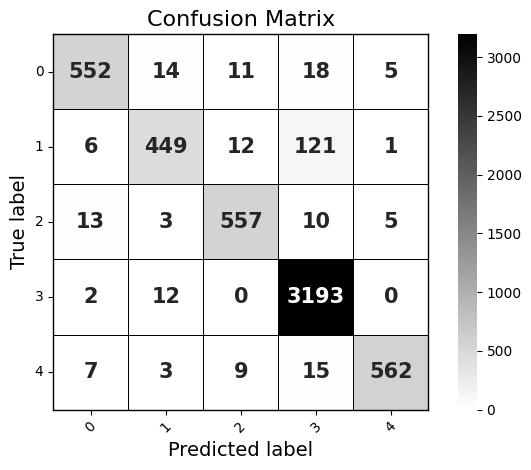
\includegraphics[width=0.7\textwidth]{Images/XG Confusion Matrix.png}  
    \caption{Confusion Matrix (XGBoost)}
    \label{XGCM}  % Label for referencing the figure
\end{figure}

\begin{figure}[h!]  
    \centering
    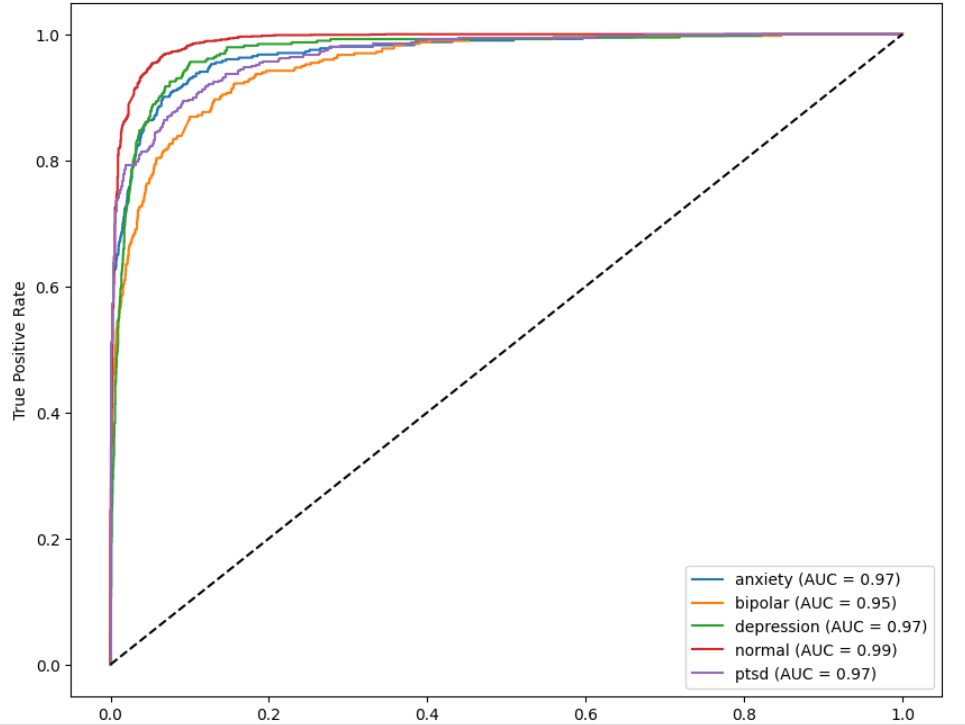
\includegraphics[width=0.7\textwidth]{Images/XG ROC.png}  
    \caption{ROC AUC (XGBoost)}
    \label{XGrOC}  % Label for referencing the figure
\end{figure}

\noindent
The XGBoost model achieved an accuracy of 87.39\%, demonstrating strong overall performance. The classification report indicates high precision and recall for the 'Normal' class, which is likely due to its substantial representation in the dataset. The 'Anxiety' and 'PTSD' classes also showed reasonable results, with the 'Anxiety' class achieving a precision of 0.81 and a recall of 0.74. However, the 'Bipolar' class exhibited a lower recall (0.62), suggesting that the model struggles more with this class. The confusion matrix highlights a well-separated 'Normal' class, while the 'Bipolar' and 'PTSD' classes experience more confusion with other categories. The ROC AUC scores further emphasize the model's good discriminatory capability, with AUC values of 0.97 for 'Anxiety,' 'Depression,' and 'PTSD,' and 0.99 for 'Normal.' These scores indicate that the model is proficient at distinguishing between different mental health conditions in the dataset.

% --------------- knn

\subsection{Results of KNN}

\begin{center}
    \textbf{KNN Classification Report} \\[0.5em]
    \begin{tabular}{|l|c|c|c|c|}
        \hline
        \textbf{Class} & \textbf{Precision} & \textbf{Recall} & \textbf{F1-Score} & \textbf{Support} \\ \hline
        Anxiety        & 0.58               & 0.31            & 0.40              & 379              \\ \hline
        Bipolar        & 0.18               & 0.59            & 0.28              & 384              \\ \hline
        Depression     & 0.47               & 0.39            & 0.43              & 373              \\ \hline
        Normal         & 0.79               & 0.69            & 0.73              & 2183             \\ \hline
        PTSD           & 0.80               & 0.09            & 0.16              & 394              \\ \hline
        \textbf{Accuracy} & \multicolumn{4}{|c|}{54.46\%} \\ \hline
        \textbf{Macro Avg} & 0.56            & 0.41            & 0.40              & 3713             \\ \hline
        \textbf{Weighted Avg} & 0.67         & 0.54            & 0.56              & 3713             \\ \hline
    \end{tabular}
\end{center}

\vspace{0.25em}
\pagebreak
\begin{center}
    \textbf{ROC Curve Areas for Each Class} \\[0.5em]
    \begin{tabular}{|l|c|}
        \hline
        \textbf{Class}  & \textbf{ROC AUC} \\ \hline
        Anxiety         & 0.73            \\ \hline
        Bipolar         & 0.67            \\ \hline
        Depression      & 0.77            \\ \hline
        Normal          & 0.80            \\ \hline
        PTSD            & 0.67            \\ \hline
    \end{tabular}
\end{center}

\vspace{0.25em}

\begin{figure}[h!]  
    \centering
    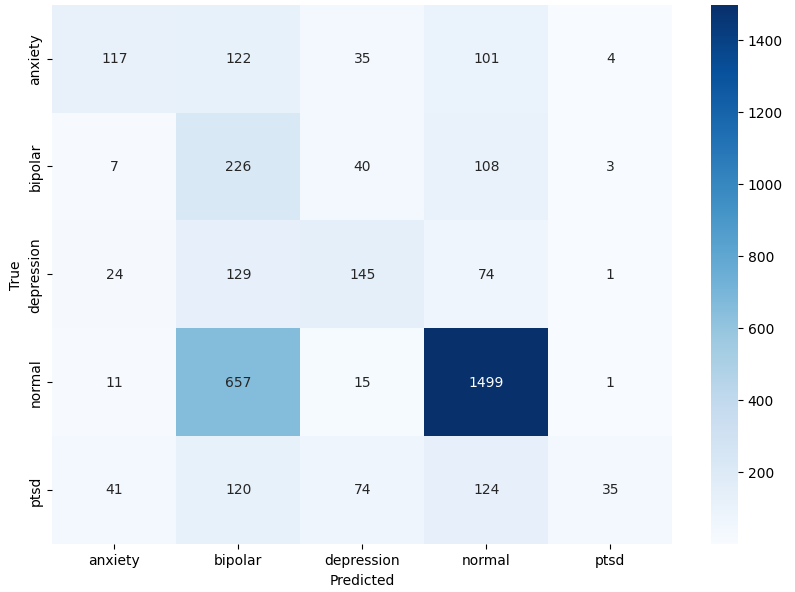
\includegraphics[width=0.7\textwidth]{Images/KNN Confusion Matrix.png}  
    \caption{Confusion Matrix (KNN)}
    \label{KNNCM}  % Label for referencing the figure
\end{figure}

\begin{figure}[h!]  
    \centering
    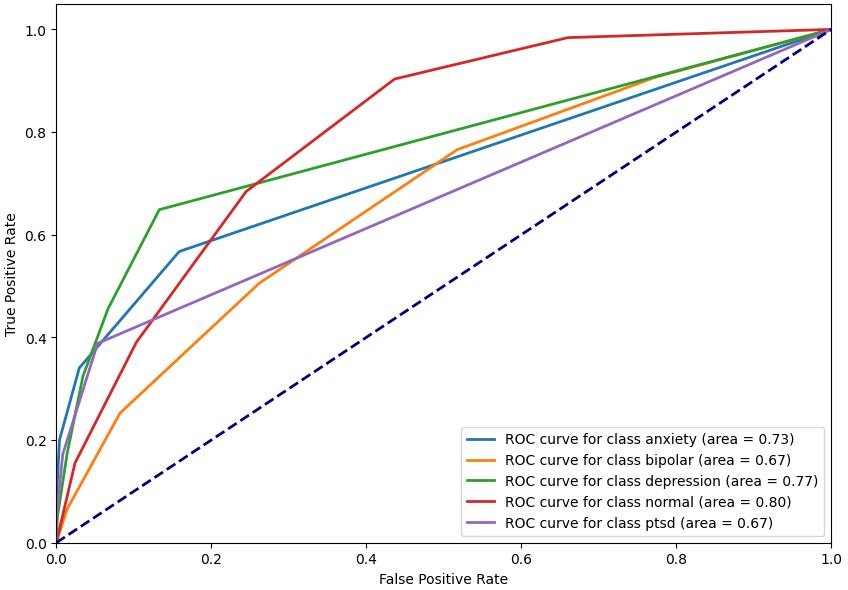
\includegraphics[width=0.7\textwidth]{Images/KNN ROC.png}  
    \caption{ROC AUC (KNN)}
    \label{KNnROC}  % Label for referencing the figure
\end{figure}

\noindent
The KNN model achieved an accuracy of 54.46\%, which is considerably lower than the XGBoost model. The classification report reveals a significant imbalance in performance across classes. The 'Normal' class achieved relatively high precision (0.79) and recall (0.69), reflecting the model's tendency to perform well with dominant classes. However, the 'Anxiety' and 'PTSD' classes performed poorly, especially with PTSD having a very low recall of 0.09, indicating substantial misclassification. The confusion matrix suggests that the model struggles with distinguishing between some classes, especially 'Anxiety' and 'Bipolar,' where confusion with other categories is high. The ROC AUC scores are relatively lower compared to the XGBoost model, with 'Normal' having the highest AUC of 0.80. These results indicate that while the KNN model offers a lower overall performance, it still provides a reasonable level of discrimination for the 'Normal' class.

\pagebreak
% ------ lstm

\subsection{Results of LSTM}

\begin{center}
    \textbf{LSTM Classification Report} \\[0.5em]
    \begin{tabular}{|l|c|c|c|c|}
        \hline
        \textbf{Class} & \textbf{Precision} & \textbf{Recall} & \textbf{F1-Score} & \textbf{Support} \\ \hline
        Anxiety        & 0.74               & 0.72            & 0.73              & 1999             \\ \hline
        Bipolar        & 0.66               & 0.70            & 0.68              & 1964             \\ \hline
        Depression     & 0.68               & 0.69            & 0.69              & 1959             \\ \hline
        Normal         & 0.97               & 0.94            & 0.95              & 10688            \\ \hline
        PTSD           & 0.72               & 0.78            & 0.75              & 1987             \\ \hline
        \textbf{Accuracy} & \multicolumn{4}{|c|}{84.91\%} \\ \hline
        \textbf{Macro Avg} & 0.75            & 0.77            & 0.76              & 18597            \\ \hline
        \textbf{Weighted Avg} & 0.85         & 0.85            & 0.85              & 18597            \\ \hline
    \end{tabular}
\end{center}

\vspace{0.1em}

\begin{center}
    \textbf{ROC Curve Areas for Each Class} \\[0.5em]
    \begin{tabular}{|l|c|}
        \hline
        \textbf{Class}  & \textbf{ROC AUC} \\ \hline
        Anxiety         & 0.95            \\ \hline
        Bipolar         & 0.92            \\ \hline
        Depression      & 0.95            \\ \hline
        Normal          & 0.98            \\ \hline
        PTSD            & 0.95            \\ \hline
    \end{tabular}
\end{center}

\vspace{0.1em}

\begin{figure}[h!]  
    \centering
    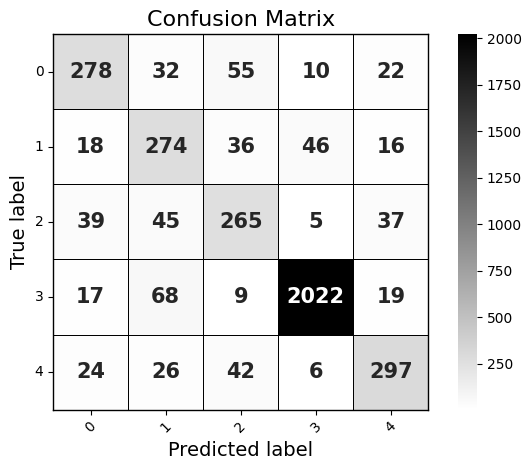
\includegraphics[width=0.7\textwidth]{Images/LSTM Confusion Matrix.png}  
    \caption{Confusion Matrix (LSTM)}
    \label{LSTMCM}  % Label for referencing the figure
\end{figure}

\begin{figure}[h!]  
    \centering
    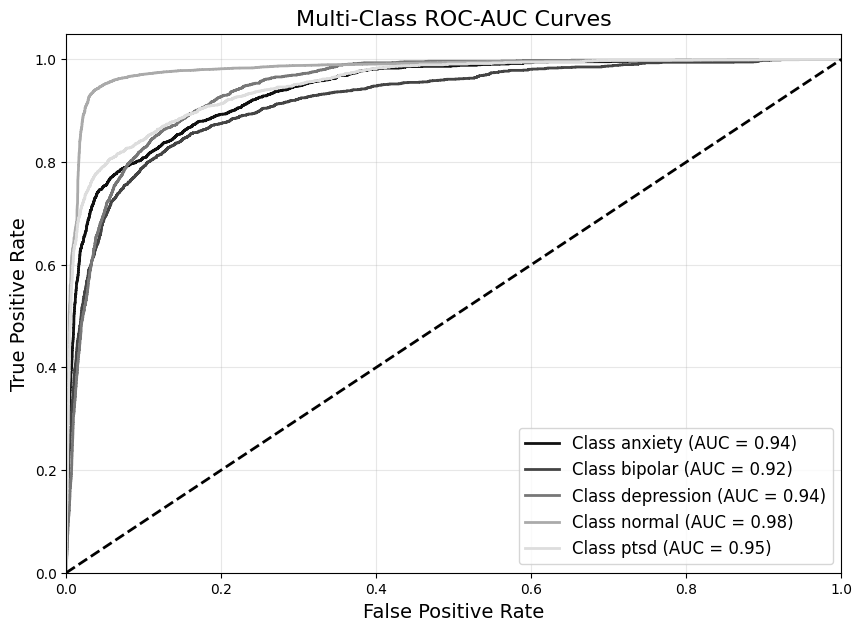
\includegraphics[width=0.7\textwidth]{Images/LSTM ROC.png}  
    \caption{ROC AUC (LSTM)}
    \label{LSTMROC}  % Label for referencing the figure
\end{figure}

\noindent
The LSTM model achieved an accuracy of 84.91\%, indicating strong performance. The classification report shows high precision, recall, and F1-scores for the 'Normal' class, which dominates the dataset. The 'Anxiety' class has reasonable performance, with a precision of 0.74 and recall of 0.72, while the 'Bipolar' and 'PTSD' classes have slightly lower precision and recall. The 'Bipolar' class shows a precision of 0.66 and recall of 0.70, while 'PTSD' has a precision of 0.72 and recall of 0.78. The confusion matrix reflects this, with 'Bipolar' and 'PTSD' misclassified with other classes, while 'Normal' is well-separated. The ROC AUC scores highlight the model's ability to distinguish between classes effectively, with 'Normal' scoring the highest.


% ----------- hyperparameter tuning

\subsection{Results of Hyperparameter Tuning}

\subsubsection{Logistic Regression}
\begin{center}
    \textbf{Hyperparameter Tuning on Logistic Regression} \\[0.5em]
    \begin{tabular}{|l|c|}
        \hline
        \textbf{Best Hyperparameters}  & \textbf{Value} \\ \hline
        Solver                        & liblinear      \\ \hline
        Penalty                       & l2             \\ \hline
        C                              & 1              \\ \hline
    \end{tabular}
\end{center}

\begin{center}
    \textbf{Classification Report} \\[0.5em]
    \begin{tabular}{|l|c|c|c|c|}
        \hline
        \textbf{Class} & \textbf{Precision} & \textbf{Recall} & \textbf{F1-Score} & \textbf{Support} \\ \hline
        Anxiety        & 0.83               & 0.77            & 0.80              & 379             \\ \hline
        Bipolar        & 0.74               & 0.55            & 0.64              & 384             \\ \hline
        Depression     & 0.76               & 0.76            & 0.76              & 373             \\ \hline
        Normal         & 0.92               & 0.99            & 0.95              & 2183            \\ \hline
        PTSD           & 0.87               & 0.77            & 0.82              & 394             \\ \hline
        \textbf{Accuracy} & \multicolumn{4}{|c|}{87.72\%} \\ \hline
        \textbf{Macro Avg} & 0.83            & 0.77            & 0.79              & 3713            \\ \hline
        \textbf{Weighted Avg} & 0.87         & 0.88            & 0.87              & 3713            \\ \hline
    \end{tabular}
\end{center}


\begin{center}
    \textbf{ROC Curve Areas for Each Class} \\[0.5em]
    \begin{tabular}{|l|c|}
        \hline
        \textbf{Class}  & \textbf{ROC AUC} \\ \hline
        Anxiety         & 0.95            \\ \hline
        Bipolar         & 0.92            \\ \hline
        Depression      & 0.96            \\ \hline
        Normal          & 0.99            \\ \hline
        PTSD            & 0.95            \\ \hline
    \end{tabular}
\end{center}

\begin{figure}[h!]  
    \centering
    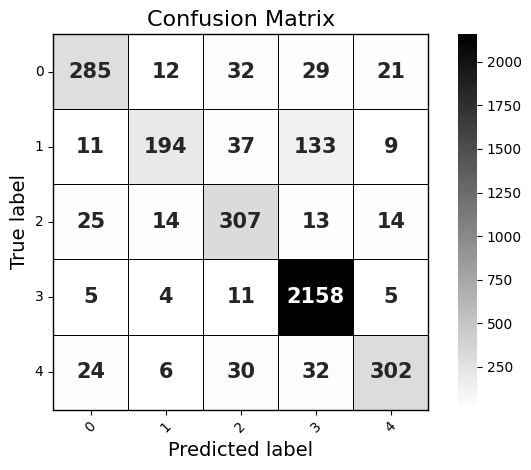
\includegraphics[width=0.9\textwidth]{Images/HP LR CM.png}  
    \caption{Classification Matrix after Hyperparameter Tuning (Logistic Regression)}
    \label{LSTMROC2}  % Label for referencing the figure
\end{figure}

\begin{figure}[h!]  
    \centering
    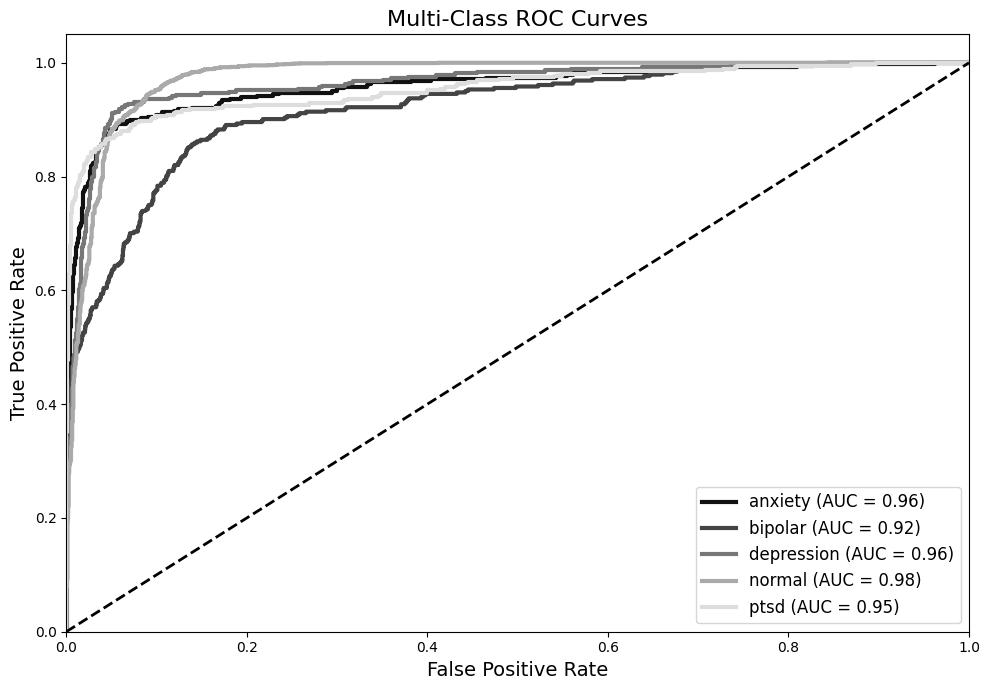
\includegraphics[width=0.9\textwidth]{Images/HP LR ROC.png}  
    \caption{ROC AUC after Hyperparamter Tuning (Logistic Regression)}
    \label{LSTMROC3}  % Label for referencing the figure
\end{figure}

\noindent
The results of hyperparameter tuning on the Logistic Regression model show that the best hyperparameters were a solver of \texttt{liblinear}, a penalty of \texttt{l2}, and a regularization parameter (\texttt{C}) of 1. The model achieved an overall accuracy of 87.72\%, with high performance across most classes. The classification report reveals that the model performs well on \texttt{normal} class with an accuracy of 92\% in predicting this class, whereas performance on \texttt{bipolar} is slightly lower \(64\% F1-score\). The ROC AUC scores indicate that the model is highly effective in distinguishing between different classes, with \texttt{normal} achieving a near-perfect AUC of 0.99, followed closely by \texttt{depression} at 0.96. These results suggest that the model is well-tuned, particularly for classes like \texttt{normal} and \texttt{anxiety}.

\pagebreak

% ----------- knn hpt
\subsubsection{K-Nearest Neighbours}
\begin{center}
    \textbf{Hyperparameter Tuning on k-NN} \\[0.5em]
    \begin{tabular}{|l|c|}
        \hline
        \textbf{Best Hyperparameters}  & \textbf{Value} \\ \hline
        Weights                       & distance       \\ \hline
        n\_neighbors                  & 10             \\ \hline
        Metric                        & euclidean      \\ \hline
    \end{tabular}
\end{center}

\begin{center}
    \textbf{Classification Report} \\[0.5em]
    \begin{tabular}{|l|c|c|c|c|}
        \hline
        \textbf{Class} & \textbf{Precision} & \textbf{Recall} & \textbf{F1-Score} & \textbf{Support} \\ \hline
        Anxiety        & 0.73               & 0.23            & 0.35              & 379             \\ \hline
        Bipolar        & 0.18               & 0.60            & 0.27              & 384             \\ \hline
        Depression     & 0.47               & 0.40            & 0.43              & 373             \\ \hline
        Normal         & 0.74               & 0.65            & 0.69              & 2183            \\ \hline
        PTSD           & 0.83               & 0.10            & 0.18              & 394             \\ \hline
        \textbf{Accuracy} & \multicolumn{4}{|c|}{52.03\%} \\ \hline
        \textbf{Macro Avg} & 0.59            & 0.40            & 0.39              & 3713            \\ \hline
        \textbf{Weighted Avg} & 0.66         & 0.52            & 0.53              & 3713            \\ \hline
    \end{tabular}
\end{center}

\begin{center}
    \textbf{ROC Curve Areas for Each Class} \\[0.5em]
    \begin{tabular}{|l|c|}
        \hline
        \textbf{Class}  & \textbf{ROC AUC} \\ \hline
        Anxiety         & 0.77            \\ \hline
        Bipolar         & 0.67            \\ \hline
        Depression      & 0.79            \\ \hline
        Normal          & 0.79            \\ \hline
        PTSD            & 0.71            \\ \hline
    \end{tabular}
\end{center}

\begin{figure}[h!]  
    \centering
    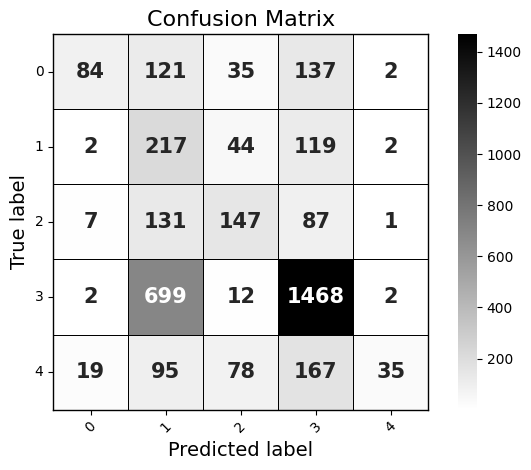
\includegraphics[width=0.9\textwidth]{Images/HP KNN CM.png}  
    \caption{Classification Matrix after Hyperparameter Tuning (KNN)}
    \label{LSTMROC4}  % Label for referencing the figure
\end{figure}

\begin{figure}[h!]  
    \centering
    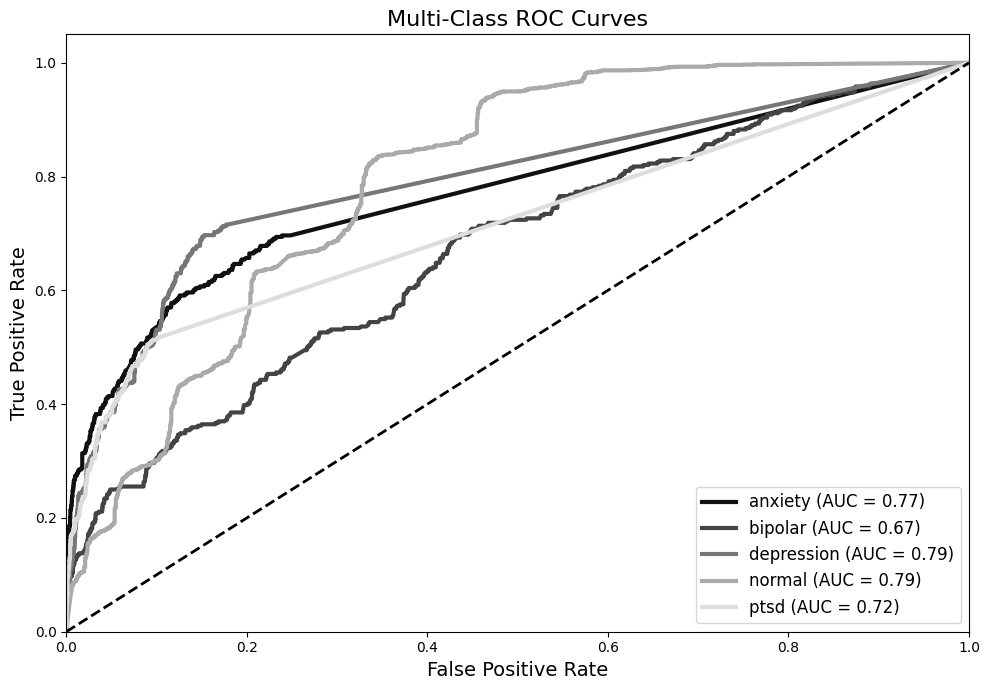
\includegraphics[width=0.9\textwidth]{Images/HP KNN ROC.png}  
    \caption{ROC AUC after Hyperparameter Tuning (KNN)}
    \label{LSTMROC5}  % Label for referencing the figure
\end{figure}

\noindent
The results of hyperparameter tuning on the k-Nearest Neighbors (k-NN) model show that the best hyperparameters were \texttt{weights} set to \texttt{distance}, \texttt{n\_neighbors} set to 10, and \texttt{metric} set to \texttt{euclidean}. Despite these optimizations, the model achieved an overall accuracy of 52.03\%, which is relatively low. The classification report indicates that the model struggled to effectively predict the \texttt{anxiety} and \texttt{PTSD} classes, with particularly low recall values (0.23 and 0.10, respectively). However, it performed reasonably well on the \texttt{normal} class with an F1-score of 0.69. The ROC AUC scores reflect this by showing relatively poor performance for \texttt{bipolar} (0.67) and \texttt{PTSD} (0.71), while \texttt{normal} and \texttt{depression} had slightly better values at 0.79 each. These results suggest that k-NN is not the best model for this dataset, as it fails to consistently classify the minority classes effectively. 

\pagebreak
\subsubsection{Support Vector Machine}
\begin{center}
    \textbf{Hyperparameter Tuning on SVM} \\[0.5em]
    \begin{tabular}{|l|c|}
        \hline
        \textbf{Best Hyperparameters}  & \textbf{Value} \\ \hline
        Kernel                        & linear         \\ \hline
        Gamma                         & scale          \\ \hline
        C                              & 1              \\ \hline
    \end{tabular}
\end{center}

\begin{center}
    \textbf{Classification Report} \\[0.5em]
    \begin{tabular}{|l|c|c|c|c|}
        \hline
        \textbf{Class} & \textbf{Precision} & \textbf{Recall} & \textbf{F1-Score} & \textbf{Support} \\ \hline
        Anxiety        & 0.72               & 0.76            & 0.74              & 379             \\ \hline
        Bipolar        & 0.62               & 0.61            & 0.61              & 384             \\ \hline
        Depression     & 0.74               & 0.71            & 0.72              & 373             \\ \hline
        Normal         & 0.94               & 0.95            & 0.95              & 2183            \\ \hline
        PTSD           & 0.78               & 0.74            & 0.76              & 394             \\ \hline
        \textbf{Accuracy} & \multicolumn{4}{|c|}{85.13\%} \\ \hline
        \textbf{Macro Avg} & 0.76            & 0.75            & 0.76              & 3713            \\ \hline
        \textbf{Weighted Avg} & 0.85         & 0.85            & 0.85              & 3713            \\ \hline
    \end{tabular}
\end{center}


\begin{center}
    \textbf{ROC Curve Areas for Each Class} \\[0.5em]
    \begin{tabular}{|l|c|}
        \hline
        \textbf{Class}  & \textbf{ROC AUC} \\ \hline
        Anxiety         & 0.92            \\ \hline
        Bipolar         & 0.88            \\ \hline
        Depression      & 0.95            \\ \hline
        Normal          & 0.98            \\ \hline
        PTSD            & 0.94            \\ \hline
    \end{tabular}
\end{center}

\begin{figure}[h!]  
    \centering
    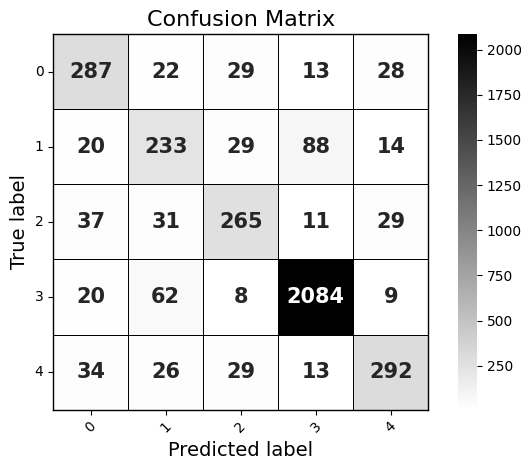
\includegraphics[width=0.9\textwidth]{Images/HP SVM CM.png}  
    \caption{Classification Matrix after Hyperparameter Tuning (SVM)}
    \label{LSTMROC6}  % Label for referencing the figure
\end{figure}

\begin{figure}[h!]  
    \centering
    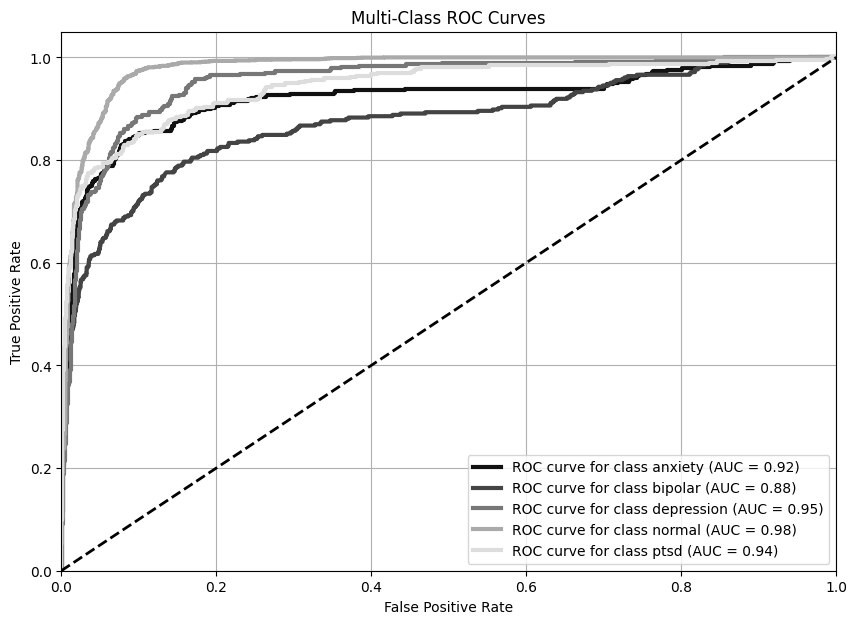
\includegraphics[width=0.9\textwidth]{Images/HP SVM ROC.png}  
    \caption{ROC AUC after Hyperparameter Tuning (SVM)}
    \label{LSTMROC}  % Label for referencing the figure
\end{figure}

\noindent
The results of hyperparameter tuning on the Support Vector Machine (SVM) model reveal that the best hyperparameters were \texttt{kernel} set to \texttt{linear}, \texttt{gamma} set to \texttt{scale}, and \texttt{C} set to 1. With these settings, the model achieved an overall accuracy of 85.13\%. The classification report indicates solid performance across most classes, with \texttt{normal} achieving the highest F1-score of 0.95, followed by \texttt{depression} at 0.72 and \texttt{anxiety} at 0.74. The \texttt{bipolar} class had a slightly lower F1-score of 0.61, indicating that the model was less effective in distinguishing this class. The ROC AUC values were strong for most classes, with \texttt{normal} reaching 0.98 and \texttt{depression}, \texttt{PTSD}, and \texttt{anxiety} all scoring above 0.90, showing that the SVM model effectively discriminates between the classes. Overall, the SVM model performed well on this dataset, particularly for the \texttt{normal} and \texttt{anxiety} classes, making it a strong contender for mental health issue classification.


\pagebreak
\subsubsection{Naive Bayes}
\begin{center}
    \textbf{Hyperparameter Tuning on Naive Bayes} \\[0.5em]
    \begin{tabular}{|l|c|}
        \hline
        \textbf{Best Hyperparameters}  & \textbf{Value} \\ \hline
        Alpha                         & 0.2914180608409973 \\ \hline
    \end{tabular}
\end{center}

\begin{center}
    \textbf{Classification Report} \\[0.5em]
    \begin{tabular}{|l|c|c|c|c|}
        \hline
        \textbf{Class} & \textbf{Precision} & \textbf{Recall} & \textbf{F1-Score} & \textbf{Support} \\ \hline
        Anxiety        & 0.69               & 0.76            & 0.72              & 379             \\ \hline
        Bipolar        & 0.75               & 0.55            & 0.64              & 384             \\ \hline
        Depression     & 0.60               & 0.83            & 0.70              & 373             \\ \hline
        Normal         & 0.96               & 0.91            & 0.94              & 2183            \\ \hline
        PTSD           & 0.73               & 0.79            & 0.76              & 394             \\ \hline
        \textbf{Accuracy} & \multicolumn{4}{|c|}{83.95\%} \\ \hline
        \textbf{Macro Avg} & 0.75            & 0.77            & 0.75              & 3713            \\ \hline
        \textbf{Weighted Avg} & 0.85         & 0.84            & 0.84              & 3713            \\ \hline
    \end{tabular}
\end{center}

\begin{center}
    \textbf{ROC Curve Areas for Each Class} \\[0.5em]
    \begin{tabular}{|l|c|}
        \hline
        \textbf{Class}  & \textbf{ROC AUC} \\ \hline
        Anxiety         & 0.93            \\ \hline
        Bipolar         & 0.93            \\ \hline
        Depression      & 0.93            \\ \hline
        Normal          & 0.99            \\ \hline
        PTSD            & 0.94            \\ \hline
    \end{tabular}
\end{center}

\begin{figure}[h!]  
    \centering
    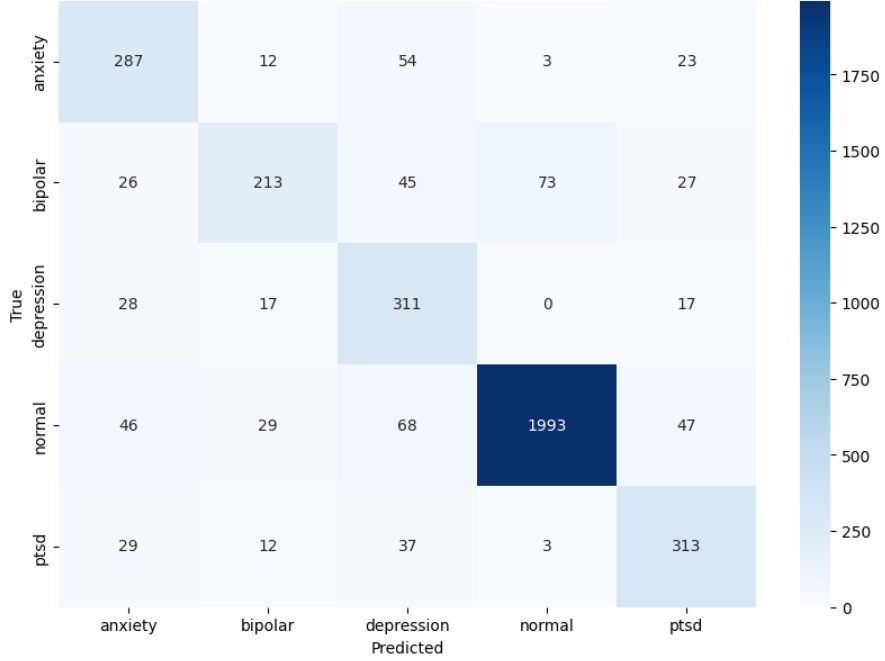
\includegraphics[width=0.9\textwidth]{Images/HP NB CM.png}  
    \caption{Classification Matrix after Hyperparameter Tuning (Naive Bayes)}
    \label{LSTMROC7}  % Label for referencing the figure
\end{figure}

\begin{figure}[h!]  
    \centering
    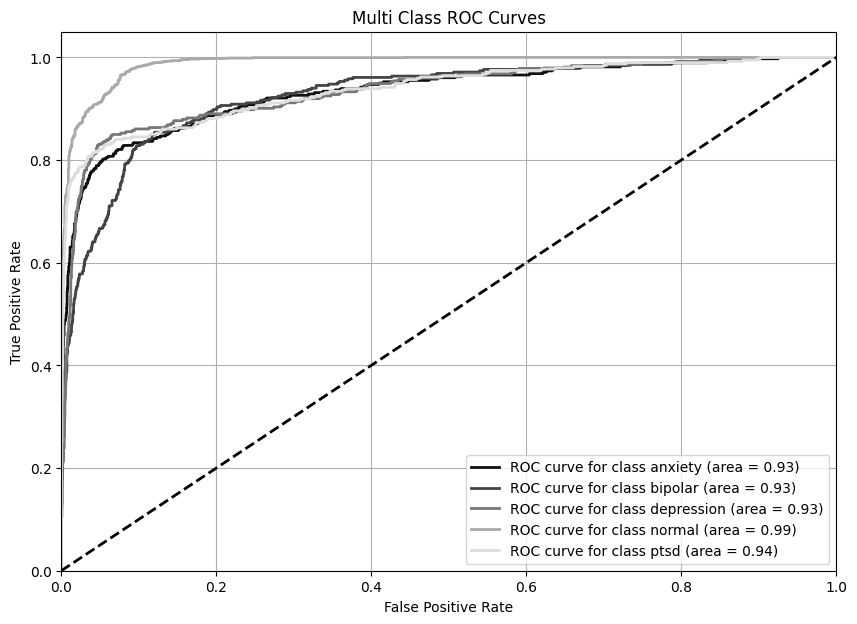
\includegraphics[width=0.9\textwidth]{Images/HP NB ROC.png}  
    \caption{ROC AUC after Hyperparameter Tuning (Naive Bayes)}
    \label{LSTMROC8}  % Label for referencing the figure
\end{figure}

\noindent
The results of hyperparameter tuning on the Naive Bayes model show that the best hyperparameter was \texttt{alpha} set to 0.2914. With this optimal value, the model achieved an accuracy of 83.95\%. The classification report reveals that the \texttt{normal} class performed the best, with a high F1-score of 0.94, followed by \texttt{PTSD} at 0.76. The \texttt{anxiety} class achieved a solid F1-score of 0.72, while \texttt{bipolar} and \texttt{depression} had lower scores. The ROC AUC curve areas demonstrate strong performance across all classes, with \texttt{normal} reaching a perfect 0.99 and the other classes scoring above 0.90. Overall, the Naive Bayes model performed well, especially in identifying \texttt{normal} and \texttt{PTSD}, making it a good candidate for mental health issue classification. After performing hyperparameter tuning using RandomizedSearchCV, Logistic Regression emerged as the best-performing model for mental health classification. The model achieved an accuracy of 87.72\%, demonstrating its strong ability to correctly classify mental health issues based on text data. The best hyperparameters found during tuning were \texttt{'solver': 'liblinear', 'penalty': 'l2', 'C': 1}, which contributed to the model's robustness and efficiency. In terms of classification performance, Logistic Regression showed a high recall and precision, especially for classes like \textit{normal}, with a recall of 0.99, indicating its proficiency in identifying the most prevalent class in the dataset. 

% -------------- Adding transformer
\subsection{Transformer based model}
\begin{center}
    \textbf{Classification Report} \\[0.5em]
    \begin{tabular}{|l|c|c|c|c|}
        \hline
        \textbf{Class} & \textbf{Precision} & \textbf{Recall} & \textbf{F1-Score} & \textbf{Support} \\ \hline
        Anxiety        & 0.75               & 0.78            & 0.76              & 379             \\ \hline
        Bipolar        & 0.76               & 0.69            & 0.73              & 384             \\ \hline
        Depression     & 0.82               & 0.72            & 0.77              & 373             \\ \hline
        Normal         & 0.95               & 0.97            & 0.96              & 2183            \\ \hline
        PTSD           & 0.79               & 0.80            & 0.79              & 394             \\ \hline
        \textbf{Accuracy} & \multicolumn{4}{|c|}{88.5\%} \\ \hline
        \textbf{Macro Avg} & 0.81            & 0.79            & 0.80              & 3713            \\ \hline
        \textbf{Weighted Avg} & 0.88         & 0.88            & 0.88              & 3713            \\ \hline
    \end{tabular}
\end{center}

\begin{center}
    \textbf{ROC Curve Areas for Each Class} \\[0.5em]
    \begin{tabular}{|l|c|}
        \hline
        \textbf{Class}  & \textbf{ROC AUC} \\ \hline
        Anxiety         & 0.97            \\ \hline
        Bipolar         & 0.94            \\ \hline
        Depression      & 0.98            \\ \hline
        Normal          & 0.99            \\ \hline
        PTSD            & 0.97            \\ \hline
    \end{tabular}
\end{center}

\begin{figure}[h!]  
    \centering
    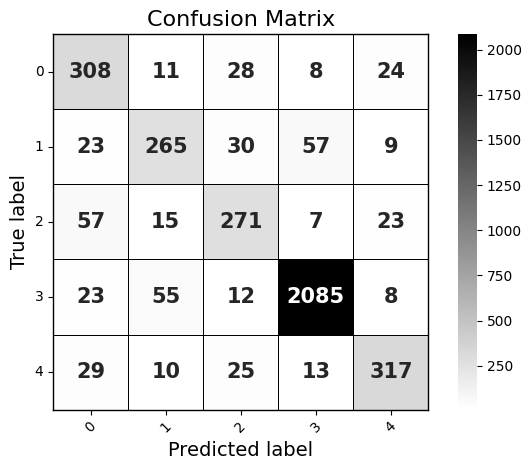
\includegraphics[width=0.75\textwidth]{Images/T CM.png}  
    \caption{Confusion Matrix for Transformer based Model}
    \label{dfdl145}  % Label for referencing the figure
\end{figure}

\begin{figure}[h!]  
    \centering
    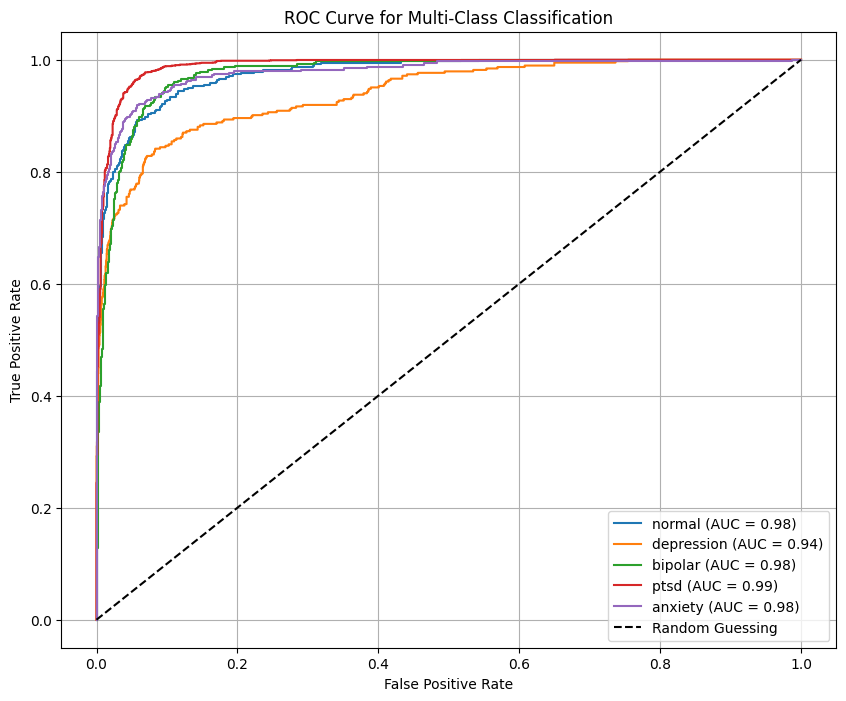
\includegraphics[width=0.75\textwidth]{Images/T ROC.png}  
    \caption{ROC AUC for Transformer based Model}
    \label{dfdl145}  % Label for referencing the figure
\end{figure}

\noindent 
The classification report and ROC AUC scores for your transformer-based model demonstrate strong performance across all classes, reflecting its ability to effectively handle the nuances of mental health text. The model achieved high precision, recall, and F1-scores, particularly for the "Normal" and "Anxiety" classes, where the precision and recall values were very high. This indicates that the model is good at identifying these conditions with minimal false positives and negatives. The high ROC AUC scores, ranging from 0.94 to 0.99 for each class, further highlight the model's ability to distinguish between different mental health conditions, with "Normal" and "Anxiety" showing particularly strong discriminatory power. The transformer-based architecture has likely contributed to these results by enabling the model to capture the complex relationships and contextual cues present in the text, which traditional models might struggle to identify. The pre-training on large datasets and fine-tuning for specific tasks has likely improved the model's ability to generalize across various mental health issues, contributing to the high accuracy of 88.5\%. This model's ability to balance performance across both major and minor classes is reflected in its macro and weighted averages, which show that it handles the class imbalance well and performs effectively on all categories. The transformer model's ability to process long-range dependencies and understand contextual relationships in the text has clearly enhanced its ability to classify mental health issues accurately, resulting in improved overall performance.

\pagebreak

\begin{figure}[h!]  
    \centering
    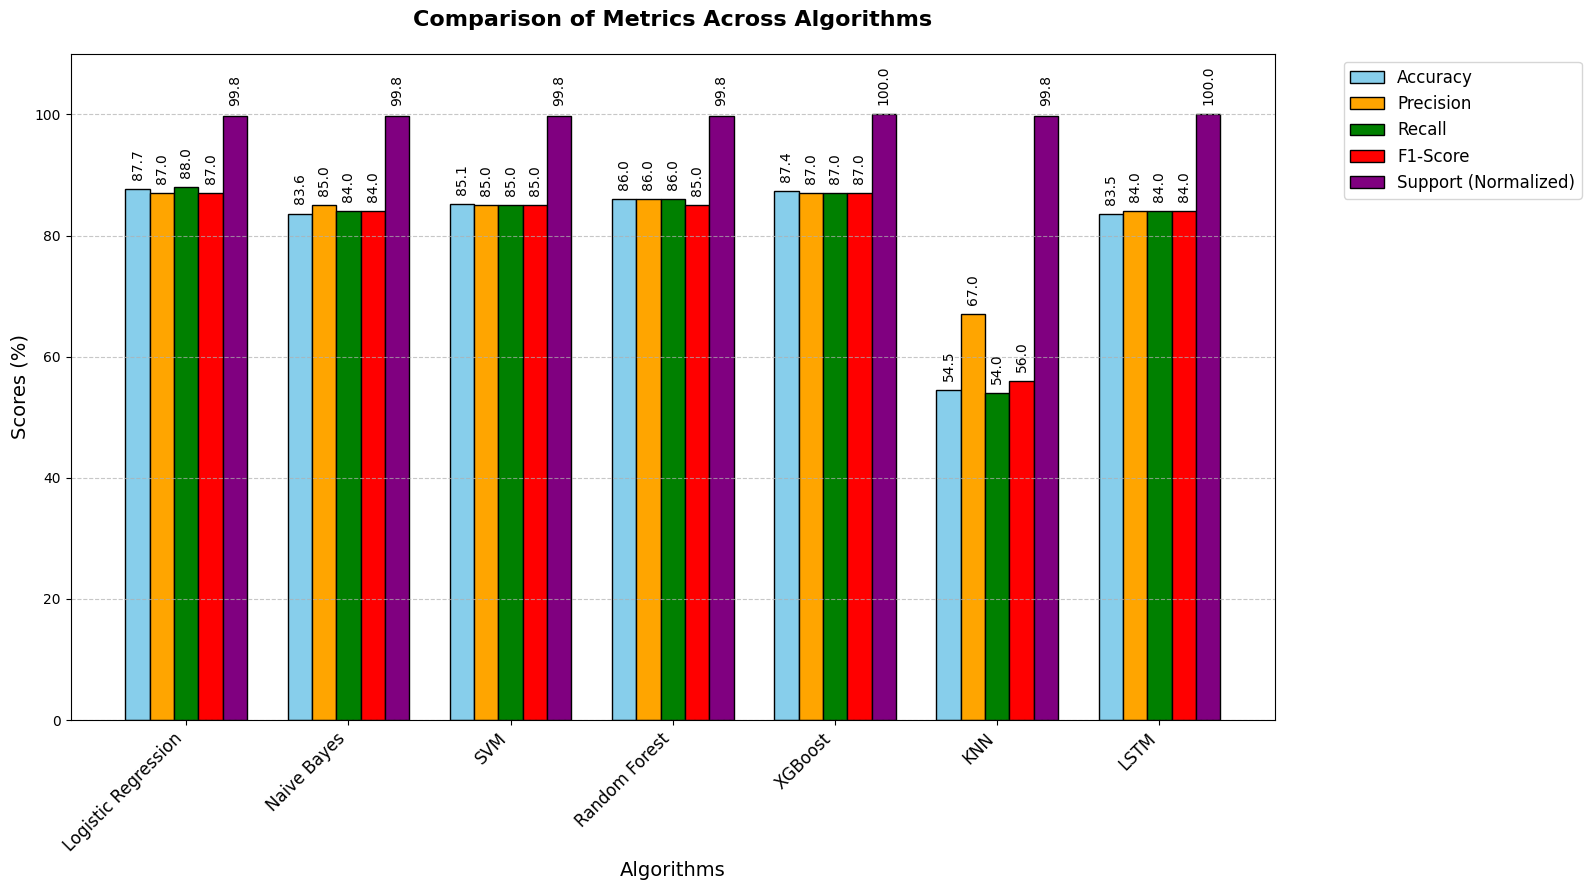
\includegraphics[width=1.0\textwidth]{Images/ML GRAPH 1.png}  
    \caption{Result Comparison of the Algorithms}
    \label{dfdl145}  % Label for referencing the figure
\end{figure}

\begin{figure}[h!]  
    \centering
    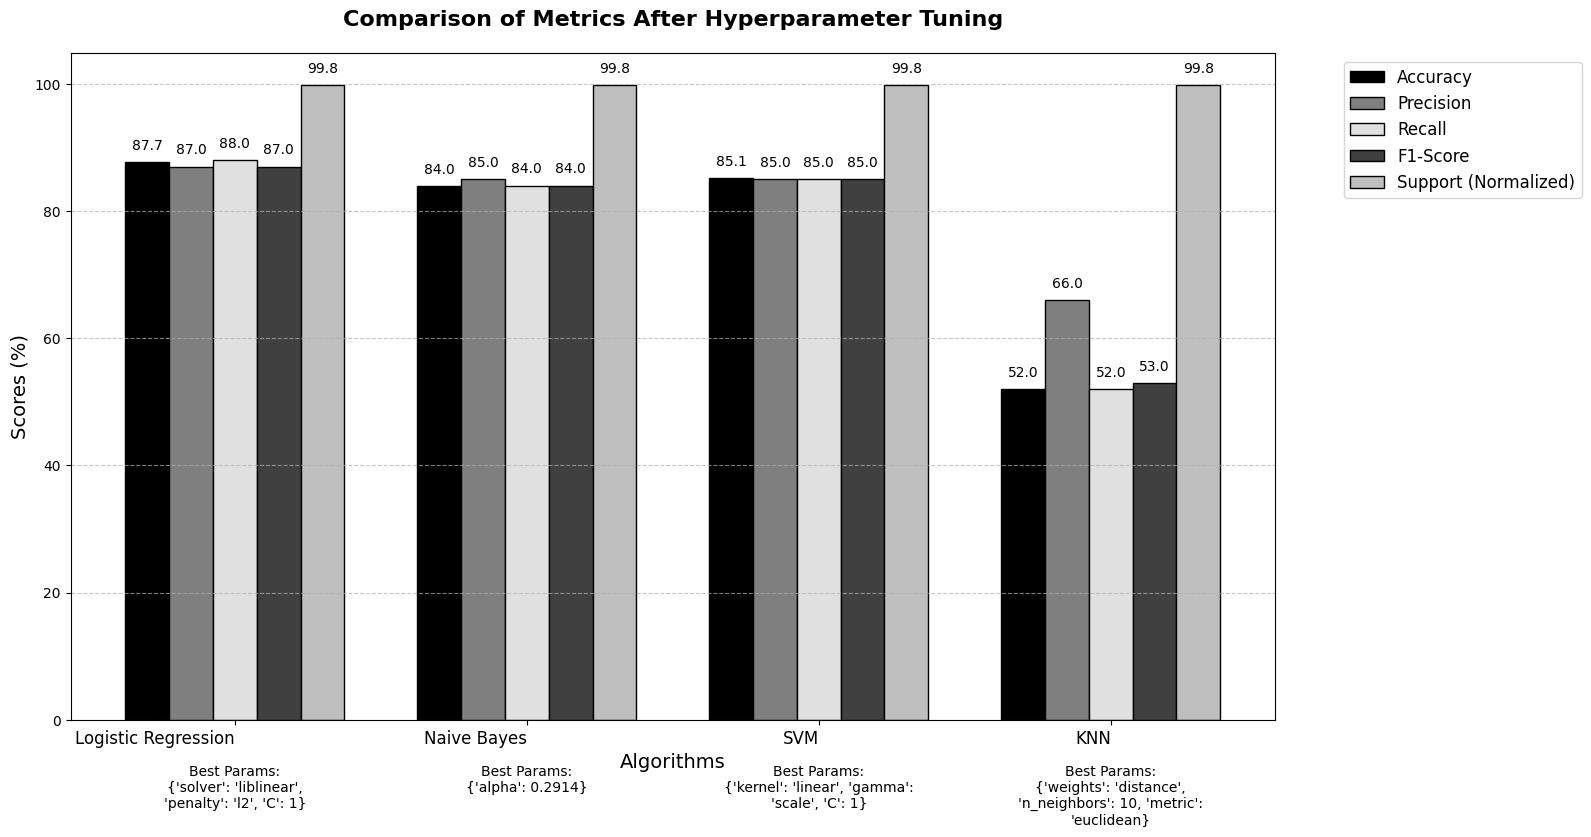
\includegraphics[width=1.0\textwidth]{Images/ML GRAPH 2 HT.png}  
    \caption{Result Comparison after Hyperparameter Tuning}
    \label{dfdl123}  % Label for referencing the figure
\end{figure}

\vspace{1em}

\noindent 
K-Nearest Neighbors (KNN) performs significantly poorly on this dataset compared to other algorithms, both before and after hyperparameter tuning. The dataset used, which includes Reddit posts with corresponding mental health labels, presents challenges for KNN due to its reliance on distance-based metrics. Specifically, KNN uses the distance between data points to classify them, but this approach is sensitive to the scale and distribution of features. In the case of text data, the feature space can be sparse and high-dimensional, making it difficult for KNN to find meaningful relationships between the posts and their associated mental health labels. After hyperparameter tuning, KNN was optimized with parameters such as \textbf{weights='distance'}, \textbf{n\_neighbors=10}, and \textbf{metric='euclidean'}, yet its performance remains suboptimal. This suggests that KNN struggles with the complexities inherent in text classification tasks, where the relationships between features (such as words or phrases in a Reddit post) are often non-linear and context-dependent. Despite tuning, the algorithm's performance metrics—accuracy, precision, recall, and F1-score—remain notably lower than those of other algorithms like Logistic Regression, Naive Bayes, or SVM. Additionally, KNN's inability to capture these subtleties in language means it performs poorly, particularly in distinguishing between categories like anxiety, bipolar disorder, or PTSD, where the text patterns may be more nuanced. Overall, KNN's reliance on proximity without considering the richer context of textual data likely contributes to its lower performance on this mental health classification task. Other algorithms, particularly those that are more suited for high-dimensional and sparse data (like Logistic Regression or SVM), show much better results as they can better account for the underlying patterns in the Reddit posts.



% ------------------ Different Vectorization ---------
\subsection{Comparison of different tokenizations}
\begin{center}
    \textbf{Model Performance Comparison} \\[0.5em]
    \begin{tabular}{|c|c|c|c|c|c|}
        \hline
        \textbf{Model} & \textbf{BoW} & \textbf{TFIDF} & \textbf{LIWC} & \textbf{Word2Vec} & \textbf{N-Gram} \\ \hline
        \textbf{Logistic Regression} & 87.66 & 86.02 & 66.36 & 79.40 & 87.13 \\ \hline
        \textbf{KNN} & 54.56 & 75.06 & 70.70 & 75.52 & 43.06 \\ \hline
        \textbf{SVC} & 85.13 & 88.26 & 68.14 & 77.89 & 84.33 \\ \hline
        \textbf{Naive Bayes} & 83.63 & 79.42 & 59.63 & 60.44 & 81.71 \\ \hline
        \textbf{Random Forest} & 85.32 & 85.73 & 76.73 & 79.88 & 79.02 \\ \hline
        \textbf{XGB} & 87.42 & 87.39 & 78.56 & 81.01 & 87.96 \\ \hline
    \end{tabular}
\end{center}

\noindent
In ensemble learning, the goal is to combine multiple base models to improve the overall performance of the system. However, using models like Logistic Regression (LR), Naive Bayes (NB), K-Nearest Neighbors (KNN), Support Vector Machine (SVM), Long Short-Term Memory (LSTM), XGBoost (XGB), and Random Forest (RF) all together as base models in an ensemble is not always feasible. Each of these models has its strengths and weaknesses, and the combination of them can lead to various challenges, particularly in terms of computational efficiency, model size, and accuracy.

\vspace{1em}

\noindent
For instance, Logistic Regression, Naive Bayes, and SVM work well with simpler vectorization methods like Bag of Words (BoW) because these methods are efficient and provide good results in terms of classification accuracy. On the other hand, more complex models like XGBoost and Random Forest can handle feature extraction methods such as TFIDF (Term Frequency-Inverse Document Frequency) better due to their ability to manage more intricate feature spaces. However, the problem arises when using these models together in a single ensemble. Although SVM with TFIDF can provide high accuracy on its own, it can negatively affect the performance of the final ensemble model. This is likely because the TFIDF features, while effective for models like SVM, may not align well with other base models, such as LR and NB, which rely more on the simpler, sparse representation of the data.

\vspace{1em}

\noindent
XGBoost, when used with N-Gram features, tends to give the highest accuracy individually, but the model size and computational demands are significantly higher, making it impractical to include in an ensemble. The larger size of the model can lead to slower inference times and increased memory usage, which is particularly problematic in real-time systems or when deploying the model at scale. Additionally, KNN is another model that is not considered as a base model in the ensemble due to its computational intensity. KNN requires the entire training dataset to be stored and does not generalize well to unseen data, and its performance deteriorates as the dataset grows, leading to slow predictions. Thus, including KNN would only further increase the computational cost and reduce the overall performance of the ensemble model.

\vspace{1em}

\noindent
Random Forest is also omitted as a base model in the ensemble for similar reasons. While Random Forest can perform well as an individual model, it is computationally intensive due to its multiple decision trees and large size, which can lead to longer training and prediction times. When included in an ensemble, its computational overhead would outweigh the benefits, especially if the ensemble consists of already complex models.

\vspace{1em}

\noindent
The reason for selecting Bag of Words (BoW) for LR, NB, and SVM, and TFIDF for XGBoost lies in the nature of these feature extraction methods and the models themselves. BoW is a simple, yet effective method for converting text data into numerical form. It represents each word as a feature in a vector space, where the value is the frequency of the word in the document. This works well for models like LR, NB, and SVM because they perform better when the features are sparse and straightforward. The simplicity of BoW ensures that these models are not overwhelmed by the sheer number of features, which helps maintain interpretability and reduces computational cost.

\vspace{1em}

\noindent
On the other hand, TFIDF takes into account not only the frequency of words in a document but also their importance in the entire corpus. Words that occur frequently across many documents are weighted lower, while words that are more specific to a particular document are given more importance. This approach is particularly useful for models like XGBoost, which can handle the more complex and rich feature sets that TFIDF generates. The increased dimensionality of TFIDF features provides a better representation of the data, which XGBoost leverages to improve accuracy. Combining BoW for LR, NB, and SVM with TFIDF for XGBoost ensures that the strengths of both simpler and more complex feature extraction methods are utilized. The simpler methods prevent the models from being overwhelmed by excessive features, while TFIDF provides more nuanced features for XGBoost, leading to improved accuracy.

\vspace{1em}

\noindent
Ultimately, the combination of \textbf{BoW} and \textbf{TFIDF} strikes a balance between simplicity and complexity, ensuring that each model works efficiently and effectively within the ensemble without causing undue computational strain. This balanced approach helps to maintain both high accuracy and manageable computational requirements, making it the best choice for feature extraction in this scenario.


\subsection{Results from Ensemble Model Training and Testing}
\subsubsection{Ensemble Model 1}

\begin{center}
    \textbf{Cross-Validation Accuracy Scores} \\[0.5em]
    \begin{tabular}{|c|c|}
        \hline
        \textbf{Cross-Validation Accuracy Scores} & \textbf{Value} \\ \hline
        1 & 0.96364126 \\ \hline
        2 & 0.95744681 \\ \hline
        3 & 0.96175599 \\ \hline
        4 & 0.95933208 \\ \hline
        5 & 0.96202532 \\ \hline
        \textbf{Mean Validation Accuracy} & \textbf{96.08\%} \\ \hline
    \end{tabular}
\end{center}


\begin{center}
    \textbf{Classification Report for Ensemble Model1} \\[0.5em]
    \begin{tabular}{|c|c|c|c|c|}
        \hline
        & \textbf{Precision} & \textbf{Recall} & \textbf{F1-Score} & \textbf{Support} \\ \hline
        \textbf{Anxiety}    & 0.97 & 0.94 & 0.95 & 400  \\ \hline
        \textbf{Bipolar}    & 0.92 & 0.85 & 0.88 & 388  \\ \hline
        \textbf{Depression} & 0.95 & 0.94 & 0.94 & 392  \\ \hline
        \textbf{Normal}     & 0.97 & 0.99 & 0.98 & 2136 \\ \hline
        \textbf{PTSD}       & 0.97 & 0.96 & 0.96 & 397  \\ \hline
        \textbf{Accuracy}   & \multicolumn{4}{|c|}{\textbf{96.08\%}} \\ \hline
        \textbf{Macro avg}  & 0.96 & 0.93 & 0.95 & 3713 \\ \hline
        \textbf{Weighted avg} & 0.96 & 0.96 & 0.96 & 3713 \\ \hline
    \end{tabular}
\end{center}

\begin{center}
    \textbf{ROC AUC Scores for Each Class} \\[0.5em]
    \begin{tabular}{|c|c|}
        \hline
        \textbf{Class} & \textbf{ROC AUC} \\ \hline
        Anxiety  & 1.0 \\ \hline
        Bipolar  & 0.99 \\ \hline
        Depression & 0.99 \\ \hline
        Normal   & 1.0 \\ \hline
        PTSD     & 0.99 \\ \hline
    \end{tabular}
\end{center}

\begin{figure}[h!]  
    \centering
    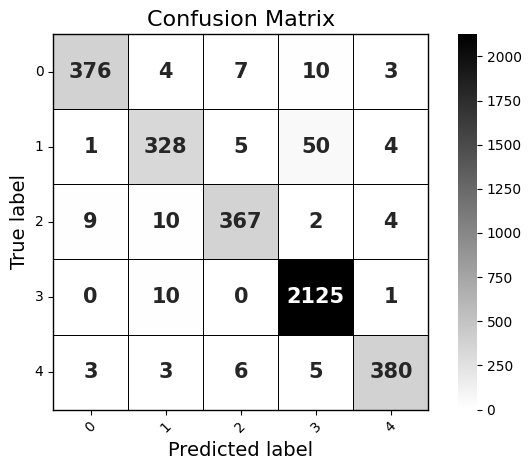
\includegraphics[width=0.7\textwidth]{Images/EM CM.png}  
    \caption{Confusion Matrix for Ensemble Model 1}
    \label{dfdl3123}  % Label for referencing the figure
\end{figure}

\begin{figure}[h!]  
    \centering
    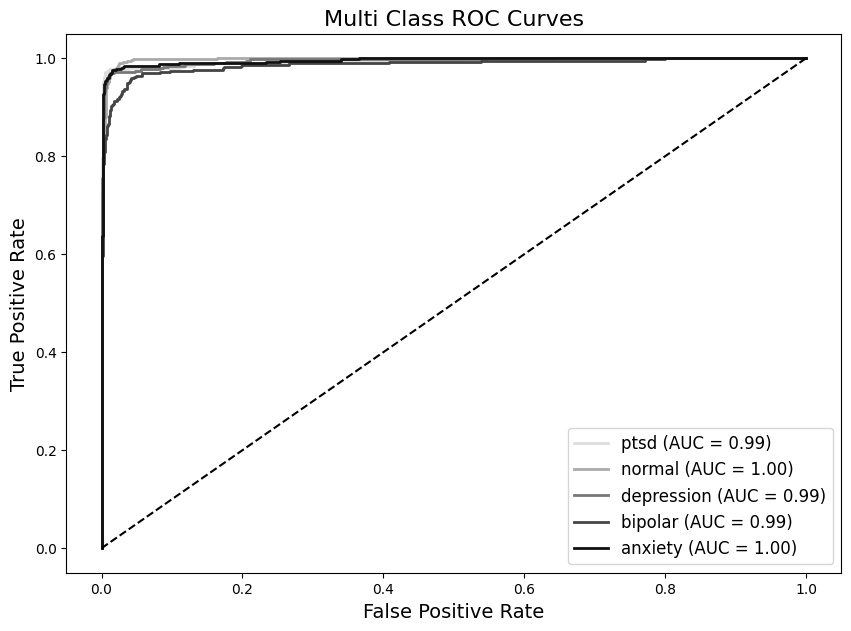
\includegraphics[width=0.7\textwidth]{Images/EM ROC.png}  
    \caption{ROC AUC Curve for Ensemble Model 1}
    \label{dfdl12443}  % Label for referencing the figure
\end{figure}


\noindent
The classification report provides an insightful summary of the ensemble model's performance, which combines Logistic Regression and XGBoost to classify mental health issues. Precision is a key metric that measures the proportion of correctly predicted positive cases out of all the positive predictions made by the model. For example, a precision of 0.97 for anxiety means that when the model predicts anxiety, it is correct 97\% of the time. Recall, on the other hand, reflects the model's ability to identify all actual positive cases in the dataset. A recall of 0.94 for anxiety suggests that the model correctly identifies 94\% of all true anxiety cases. The F1-score, which balances precision and recall, is also an important metric. With an F1-score of 0.95 for anxiety, the model strikes a good balance between precision and recall, indicating that it performs well across both metrics. Support represents the number of actual instances of a class in the dataset, and for anxiety, there are 1999 instances in the test set. The model's overall accuracy is 96.08\%, meaning that it correctly predicts the mental health condition for 96.08\% of the test instances, reflecting the overall effectiveness of the model. The macro average, which takes the unweighted mean of precision, recall, and F1-scores across all classes, shows an average precision of 0.96, recall of 0.93, and F1-score of 0.95. This provides a general idea of the model's performance across all classes without accounting for class imbalance. The weighted average, however, adjusts for the class distribution by giving more weight to classes with more instances. The weighted averages for precision, recall, and F1-score are all 0.96, reflecting strong overall performance, especially when considering the differing class sizes. The ROC AUC scores are another key performance indicator that evaluates the model's ability 

\noindent
to distinguish between different classes. The AUC score ranges from 0 to 1, with 1 representing perfect classification. A perfect AUC score of 1.0 for anxiety, normal, and PTSD indicates that the model can perfectly differentiate between these classes and others. The AUC scores for bipolar and depression are 0.99, which is almost perfect, further demonstrating the model's strong performance across all classes. Overall, these metrics indicate that the ensemble model is highly effective at classifying mental health issues, with robust precision, recall, and the ability to distinguish between the different conditions. The confusion matrix will provide insight into the number of false positives, false negatives, true positives, and true negatives for each class. By looking at the confusion matrix, you can better understand where the model might be misclassifying certain classes, such as when it confuses anxiety with depression or bipolar with PTSD. For example, a high number of false positives in the anxiety class would mean the model is often predicting anxiety when it's actually a different mental health condition. Conversely, a high number of false negatives would mean the model is missing anxiety cases. The combination of logistic regression and XGBoost allows the ensemble model to leverage the strengths of both algorithms. While logistic regression is simple and interpretable, it might struggle with non-linearities in the data. XGBoost, on the other hand, is a powerful gradient boosting algorithm that can capture complex patterns in the data. By stacking their predictions, the ensemble model benefits from both simplicity and complexity, achieving higher accuracy and robustness in text-based classification tasks.

\vspace{1em}

\noindent
This ensemble model, combining Logistic Regression and XGBoost, is highly effective for the mental health classification web application due to its ability to leverage the strengths of both algorithms. Logistic Regression provides a simple yet powerful linear approach to classification, offering interpretability and efficiency, while XGBoost excels at handling complex, non-linear relationships with its gradient boosting framework, enabling better accuracy and robustness. By stacking these models, the ensemble approach mitigates the individual weaknesses of each algorithm—Logistic Regression's limitations in capturing non-linear patterns and XGBoost's susceptibility to overfitting on small datasets—resulting in a more balanced, accurate, and generalizable model. This synergy ensures that the mental health classification web application delivers reliable, high-precision predictions across diverse text-based inputs.

\begin{figure}[h!]  
    \centering
    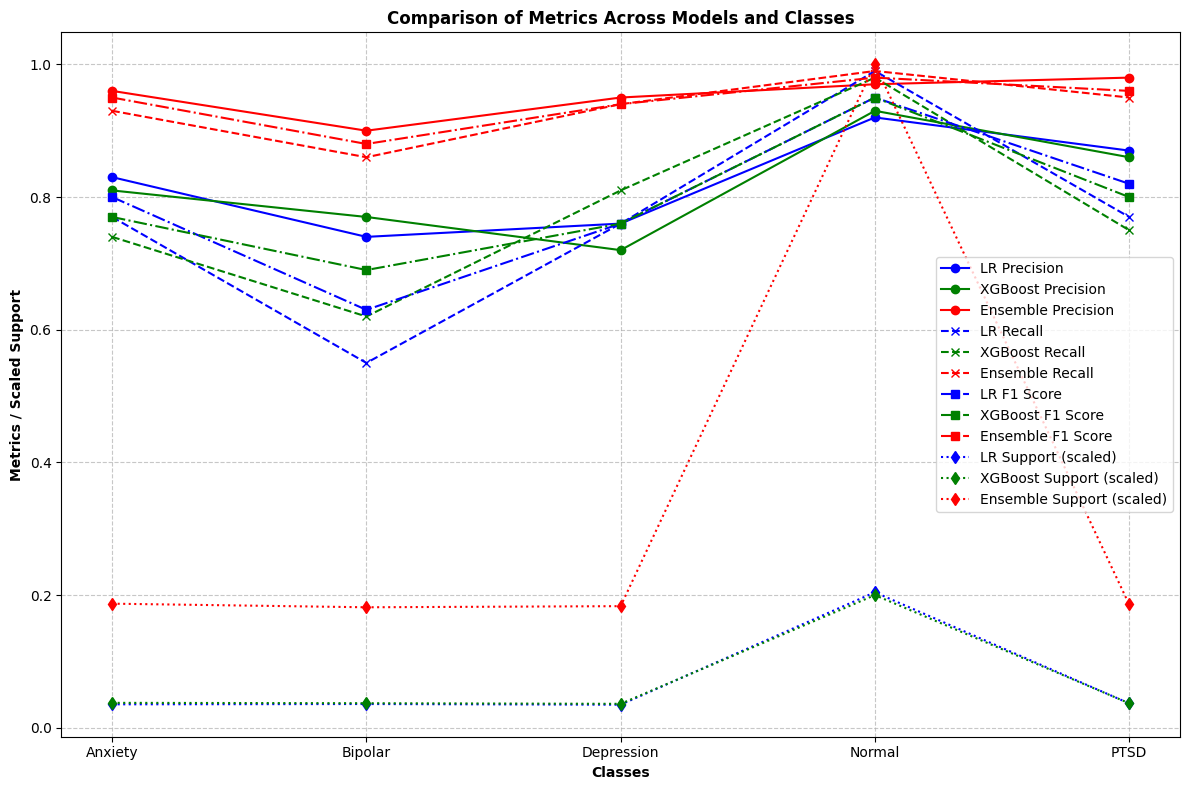
\includegraphics[width=1.0\textwidth]{Images/EM RESULT.png}  
    \caption{Comparison of Base models and Ensemble Model1}
    \label{dfdl1244883}  % Label for referencing the figure
\end{figure}

\pagebreak

\subsubsection{Ensemble Model 2}

\begin{center}
    \textbf{Cross-Validation Accuracy Scores} \\[0.5em]
    \begin{tabular}{|c|c|}
        \hline
        \textbf{Cross-Validation Accuracy Scores} & \textbf{Value} \\ \hline
        1 & 0.980878 \\ \hline
        2 & 0.97629949 \\ \hline
        3 & 0.98249394 \\ \hline
        4 & 0.97522219 \\ \hline
        5 & 0.97710746 \\ \hline
        \textbf{Mean Validation Accuracy} & \textbf{97.84\%} \\ \hline
    \end{tabular}
\end{center}


\begin{center}
    \textbf{Classification Report for Ensemble Model2} \\[0.5em]
    \begin{tabular}{|c|c|c|c|c|}
        \hline
        & \textbf{Precision} & \textbf{Recall} & \textbf{F1-Score} & \textbf{Support} \\ \hline
        \textbf{Anxiety}    & 0.97 & 0.97 & 0.97 & 400  \\ \hline
        \textbf{Bipolar}    & 0.95 & 0.92 & 0.93 & 388  \\ \hline
        \textbf{Depression} & 0.98 & 0.96 & 0.97 & 392  \\ \hline
        \textbf{Normal}     & 0.99 & 0.99 & 0.99 & 2136 \\ \hline
        \textbf{PTSD}       & 0.97 & 0.98 & 0.98 & 397  \\ \hline
        \textbf{Accuracy}   & \multicolumn{4}{|c|}{\textbf{97.93\%}} \\ \hline
        \textbf{Macro avg}  & 0.97 & 0.97 & 0.97 & 3713 \\ \hline
        \textbf{Weighted avg} & 0.98 & 0.98 & 0.98 & 3713 \\ \hline
    \end{tabular}
\end{center}

\begin{center}
    \textbf{ROC AUC Scores for Each Class} \\[0.5em]
    \begin{tabular}{|c|c|}
        \hline
        \textbf{Class} & \textbf{ROC AUC} \\ \hline
        Anxiety  & 1.0 \\ \hline
        Bipolar  & 1.0 \\ \hline
        Depression & 1.0 \\ \hline
        Normal   & 1.0 \\ \hline
        PTSD     & 1.0 \\ \hline
    \end{tabular}
\end{center}

\begin{figure}[h!]  
    \centering
    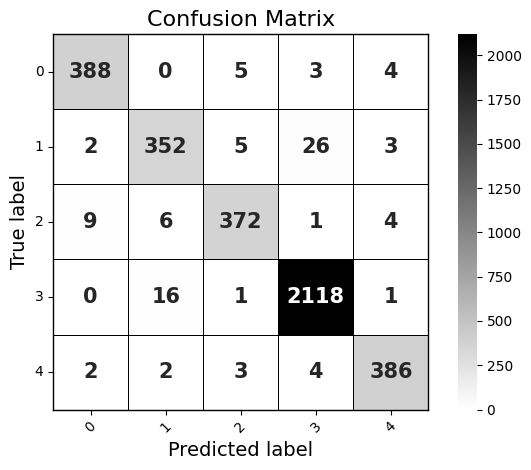
\includegraphics[width=0.7\textwidth]{Images/EM2 CM.png}  
    \caption{Confusion Matrix for Ensemble Model 2}
    \label{em2 cm}  % Label for referencing the figure
\end{figure}

\begin{figure}[h!]  
    \centering
    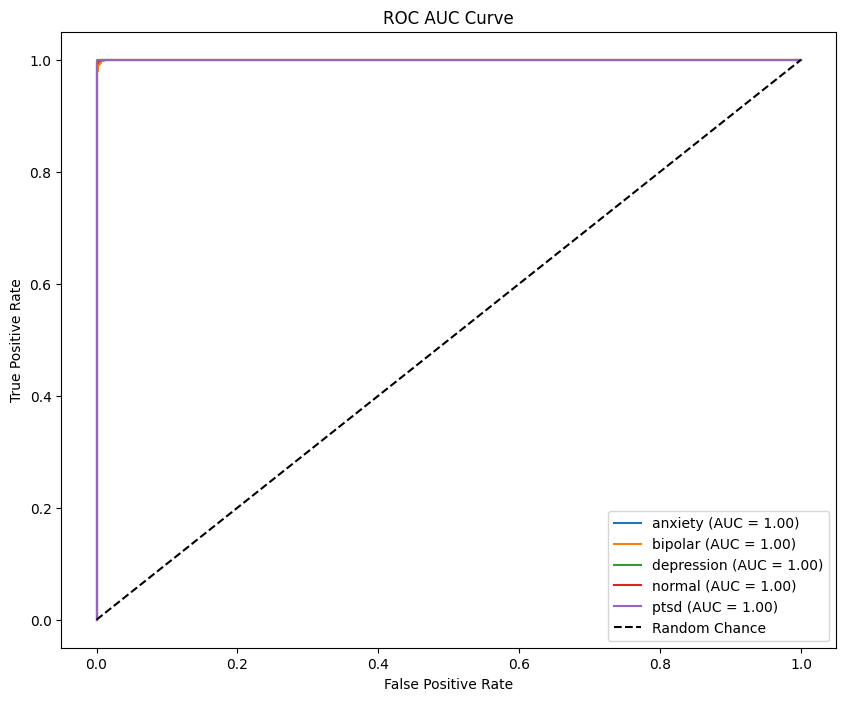
\includegraphics[width=0.7\textwidth]{Images/EM2 ROC.png}  
    \caption{ROC AUC for Ensemble Model 2}
    \label{em2 roc}  % Label for referencing the figure
\end{figure}

\begin{figure}[h!]  
    \centering
    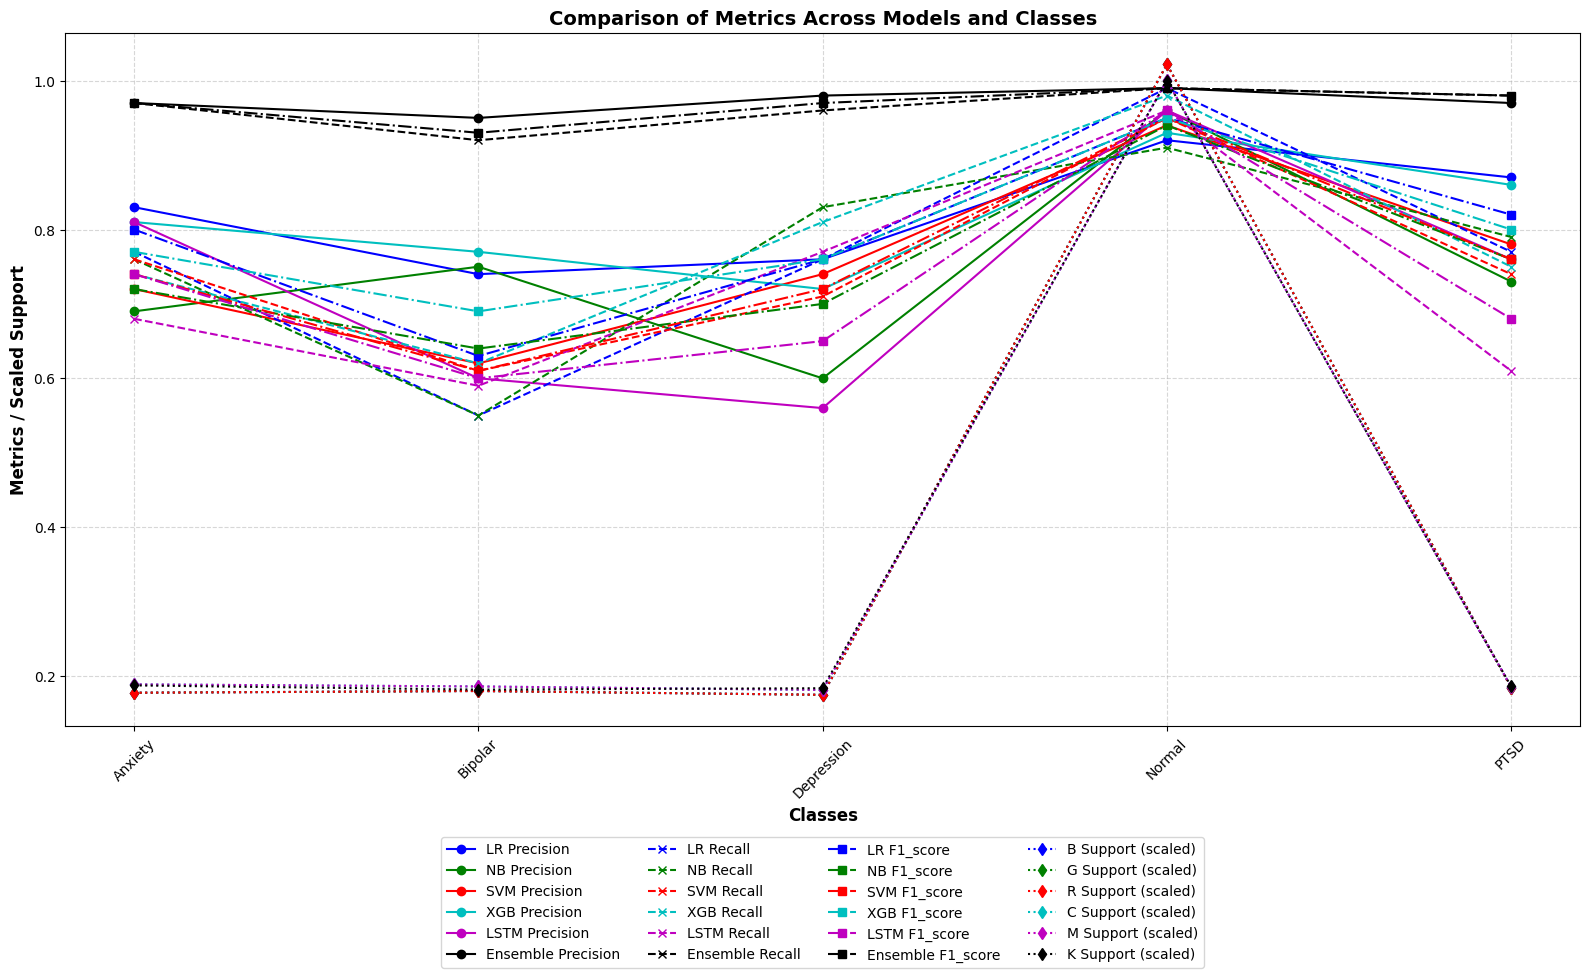
\includegraphics[width=1.0\textwidth]{Images/EM2 RESULT.png}  
    \caption{Comparison of Base models and Ensemble Model2}
    \label{lstm arch}  % Label for referencing the figure
\end{figure}

\noindent
Each row of the matrix represents the true class, while each column represents the predicted class. The diagonal elements (390, 357, 377, 2122, 390) show the number of correct predictions for each class (anxiety, bipolar, depression, normal, PTSD), while the off-diagonal elements represent misclassifications. For example, the model misclassified 2 samples from the anxiety class as depression and 1 sample from the bipolar class as normal, but overall, the model made very few misclassifications. An ROC AUC score of 1.0 indicates perfect classification performance for each class, meaning that the model has perfectly separated the classes based on the probability predictions. This reinforces the outstanding performance of the XGBoost model.

\noindent
Using XGBoost as a meta-learner in an ensemble model is a strategic decision that brings several advantages, both in terms of performance and interpretability. To understand why XGBoost is an excellent choice, it is important to first appreciate the concept of a meta-learner and how ensemble learning works. Ensemble learning involves combining multiple base models to improve prediction accuracy by leveraging their individual strengths. In a typical ensemble method, the predictions of several base models (e.g., logistic regression, SVM, Naive Bayes, LSTM) are used as input features for a meta-learner, which then learns how to best combine these predictions to make a final decision. The meta-learner's role is to determine which base model's predictions are more reliable for each sample, thus improving the overall performance of the ensemble. XGBoost, a gradient boosting algorithm, has several features that make it an ideal candidate for a meta-learner in this context. First, XGBoost is known for its ability to handle complex relationships in data, especially in terms of interactions between features. Unlike simpler models like logistic regression or Naive Bayes, XGBoost builds decision trees iteratively, where each new tree is focused on correcting the errors made by the previous trees. This iterative approach allows XGBoost to capture non-linear patterns and subtle interactions that might be missed by individual base models. When used as a meta-learner, XGBoost can intelligently combine the predictions from the base models by learning the optimal way to weigh the output of each base model. This is especially important in a multi-model setting where different classifiers might have complementary strengths—XGBoost can effectively "learn" when to trust each model's prediction more, depending on the characteristics of the input data. Another advantage of using XGBoost as a meta-learner is its regularization capabilities. XGBoost includes both L1 and L2 regularization, which helps prevent overfitting. In the context of ensemble learning, this is particularly useful because, with multiple models contributing to the final prediction, the meta-learner needs to ensure it doesn't overly rely on any one base model, especially if that model is prone to overfitting. By applying regularization, XGBoost encourages the model to generalize well, ensuring that the ensemble is robust and does not become overly sensitive to the training data or to noise.

\vspace{1em}
\noindent
Additionally, XGBoost is highly efficient in terms of both computation and memory usage. It is designed to work well with large datasets, and its ability to handle sparse data effectively makes it a good fit for a wide variety of tasks, including those involving textual data or other high-dimensional inputs. In ensemble models, where multiple base models generate a large number of features (e.g., prediction probabilities from each base model), XGBoost’s efficiency in processing these features allows it to scale well even as the number of base models or the size of the dataset grows. Another key benefit is XGBoost’s ability to handle imbalanced datasets. Many classification tasks, especially in medical or mental health data, suffer from class imbalances, where some classes (e.g., “Normal”) are more frequent than others (e.g., “Bipolar” or “PTSD”). XGBoost has built-in features to adjust for class imbalances, such as using class weights or employing custom loss functions. This is important in a meta-learner context because the base models might not be equally effective across all classes. XGBoost can ensure that the ensemble model doesn't bias its predictions toward the majority class, which is crucial for improving the overall classification performance, especially for underrepresented classes.  Furthermore, XGBoost provides excellent interpretability through feature importance scores. In an ensemble model, where several base models contribute to the final prediction, understanding how each base model influences the outcome is valuable for both improving the model and for explaining its behavior. XGBoost offers built-in tools to analyze the importance of individual features (in this case, the predictions of the base models), allowing practitioners to understand how the meta-learner is making decisions and which base models are contributing the most to its predictions. Lastly, XGBoost’s performance in various machine learning competitions has demonstrated its robustness. It is one of the top-performing algorithms in tasks such as classification and regression, often outperforming other methods, including random forests and neural networks. Its popularity and track record make it a safe and reliable choice for a meta-learner.


\vspace{1em}

\noindent
While using models like XGBoost, SVM, Naive Bayes, and LSTM as meta-learners in ensemble modeling can provide high accuracy, these models can also be prone to \textbf{overfitting}, especially when they are trained on the predictions of multiple base models. Overfitting occurs when the model learns the noise or patterns specific to the training data that do not generalize well to unseen data. For XGBoost, although it is a powerful and highly flexible model, its ability to capture complex relationships between features can lead to overfitting, especially when the base models are already strong. When combined with a large number of features from multiple base models, the XGBoost meta-learner may excessively adjust to small fluctuations in the training data, leading to high performance on the training set but poor generalization to new data. This risk is heightened if the base models already provide overlapping or correlated predictions, which can reinforce irrelevant patterns for the meta-learner. Similarly, SVM as a meta-learner can overfit in ensemble setups. SVM, especially when using a non-linear kernel, is very sensitive to the scale of features and may become highly specialized to the training data if not properly tuned. When stacking the output of multiple base models, each with its own biases and prediction tendencies, the SVM meta-learner may overemphasize specific instances that are not representative of the general data distribution. This can lead to poor performance on new, unseen data despite strong accuracy on the training set. Naive Bayes is another model that can overfit when used as a meta-learner. Although it assumes independence between features, stacking it with predictions from base models may violate this assumption, leading to overly optimistic performance during training. Naive Bayes models are particularly sensitive to correlated features, and in an ensemble, where the base models might produce similar predictions, the meta-learner might end up fitting to these correlations too closely. This results in high training accuracy but a significant drop in performance when applied to unseen data. Finally, LSTM models, although excellent at capturing long-range dependencies in sequential data, can also overfit when used as a meta-learner. LSTMs are prone to memorizing the training data, especially when the number of parameters in the model is large relative to the size of the training set. In ensemble settings, the LSTM meta-learner might overly adapt to the specific features of the training data, particularly when the base models' predictions are very similar, reinforcing the same patterns in the data. This can cause the LSTM meta-learner to perform well on training data but fail to generalize effectively to new data.

\subsubsection{Ensemble Model 3}

\begin{center}
    \textbf{Cross-Validation Accuracy Scores} \\[0.5em]
    \begin{tabular}{|c|c|}
        \hline
        \textbf{Cross-Validation Accuracy Scores} & \textbf{Value} \\ \hline
        1 & 0.98195529 \\ \hline
        2 & 0.97549152 \\ \hline
        3 & 0.98060867 \\ \hline
        4 & 0.97603016 \\ \hline
        5 & 0.97629949 \\ \hline
        \textbf{Mean Validation Accuracy} & \textbf{97.81\%} \\ \hline
    \end{tabular}
\end{center}

\begin{center}
    \textbf{Classification Report for Ensemble Model3} \\[0.5em]
    \begin{tabular}{|c|c|c|c|c|}
        \hline
        & \textbf{Precision} & \textbf{Recall} & \textbf{F1-Score} & \textbf{Support} \\ \hline
        \textbf{Anxiety}    & 0.98 & 0.97 & 0.98 & 400  \\ \hline
        \textbf{Bipolar}    & 0.96 & 0.90 & 0.93 & 388  \\ \hline
        \textbf{Depression} & 0.97 & 0.96 & 0.96 & 392  \\ \hline
        \textbf{Normal}     & 0.98 & 1.00 & 0.99 & 2136 \\ \hline
        \textbf{PTSD}       & 0.97 & 0.97 & 0.97 & 397  \\ \hline
        \textbf{Accuracy}   & \multicolumn{4}{|c|}{\textbf{97.76\%}} \\ \hline
        \textbf{Macro avg}  & 0.97 & 0.96 & 0.97 & 3713 \\ \hline
        \textbf{Weighted avg} & 0.98 & 0.98 & 0.98 & 3713 \\ \hline
    \end{tabular}
\end{center}

\pagebreak

\begin{center}
    \textbf{ROC AUC Scores} \\[0.5em]
    \begin{tabular}{|c|c|}
        \hline
        \textbf{Anxiety} & 1.00 \\ \hline
        \textbf{Bipolar} & 1.00 \\ \hline
        \textbf{Depression} & 1.00 \\ \hline
        \textbf{Normal} & 1.00 \\ \hline
        \textbf{PTSD} & 1.00 \\ \hline
    \end{tabular}
\end{center}

\begin{figure}[h!]  
    \centering
    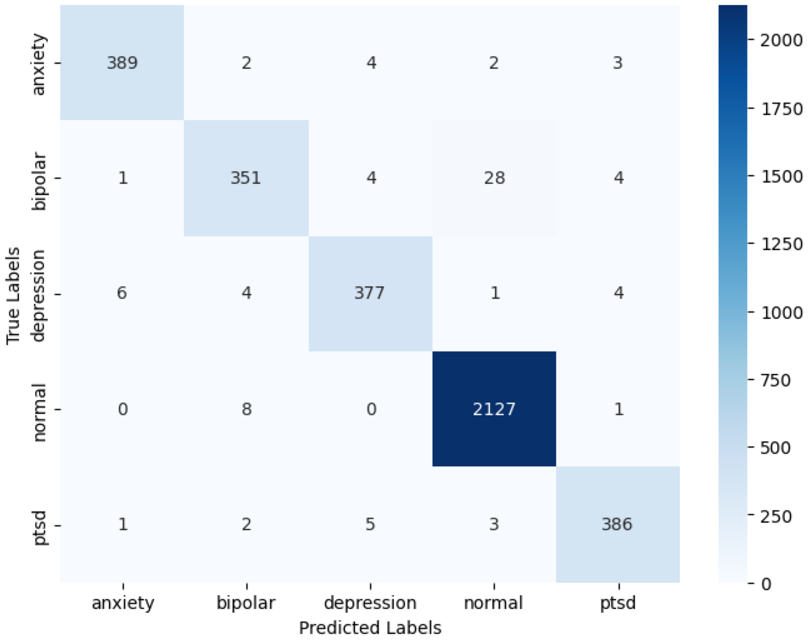
\includegraphics[width=0.7\textwidth]{Images/EM3 CM.png}  
    \caption{Confusion Matrix for Ensemble Model 3}
    \label{lstm arch}  % Label for referencing the figure
\end{figure}

\begin{figure}[h!]  
    \centering
    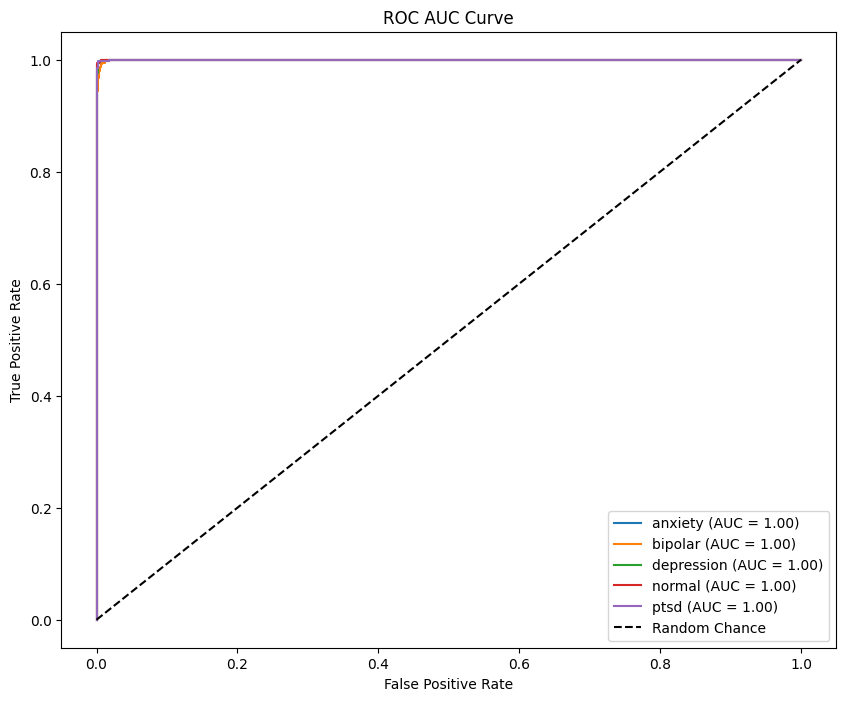
\includegraphics[width=0.7\textwidth]{Images/EM3 ROC.png}  
    \caption{ROC AUC for Ensemble Model 3}
    \label{lstm arch}  % Label for referencing the figure
\end{figure}

\begin{figure}[h!]  
    \centering
    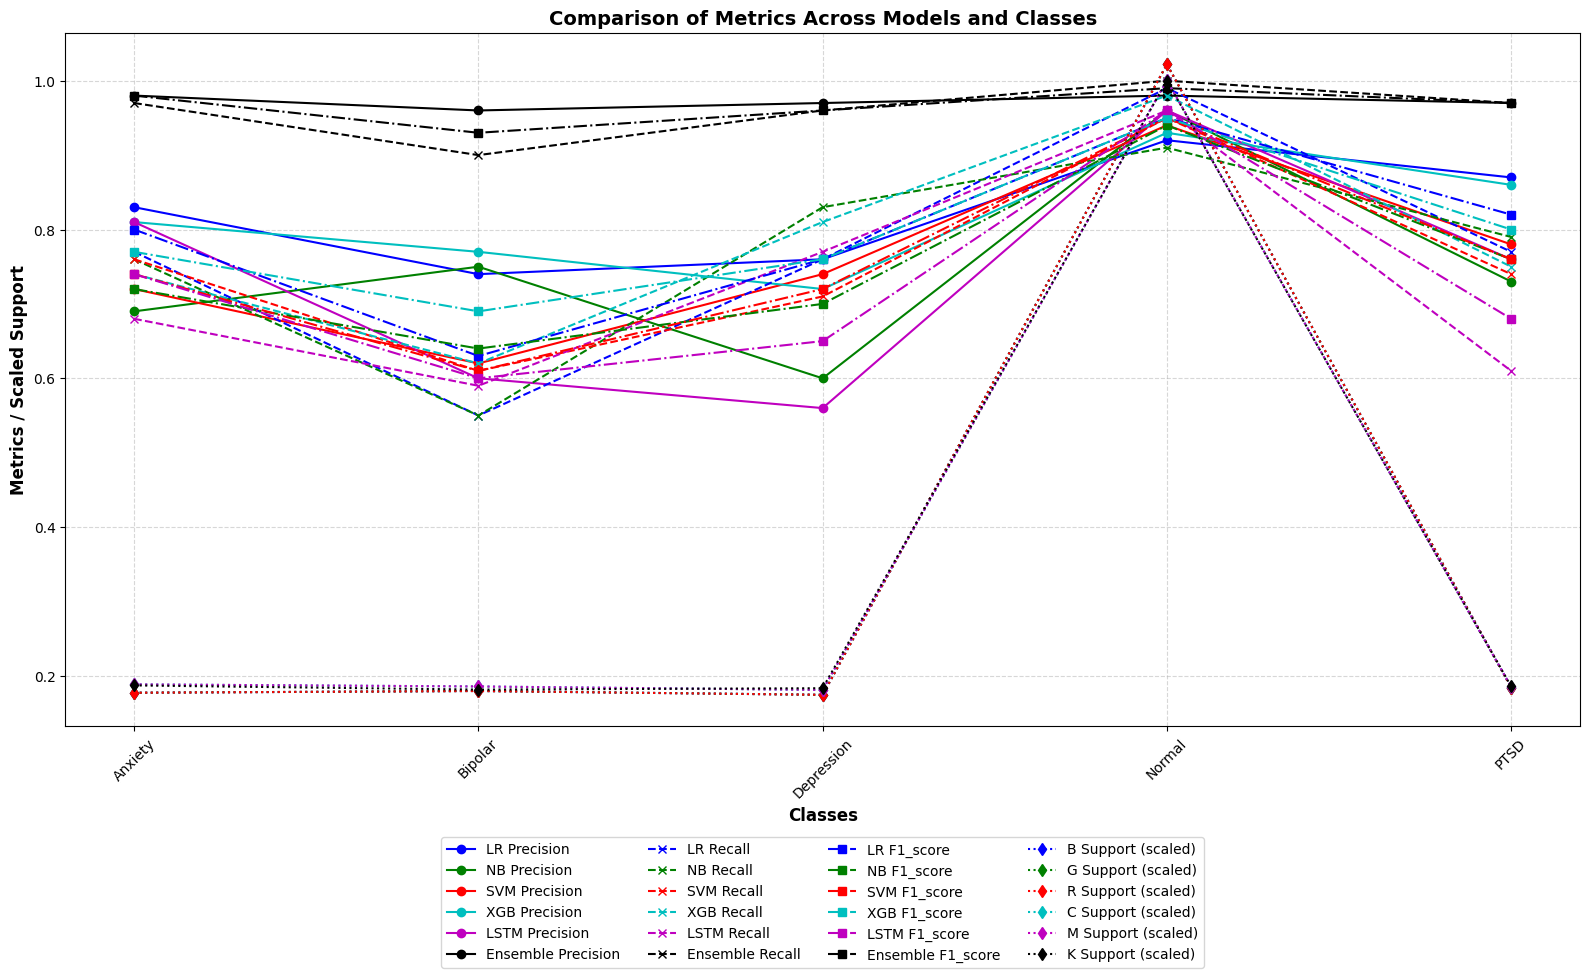
\includegraphics[width=1.0\textwidth]{Images/EM3 RESULT.png}  
    \caption{Comparison of Base Models and Ensemble Model3}
    \label{lstm arch}  % Label for referencing the figure
\end{figure}

\noindent
The confusion matrix for the Random Forest model shows the performance of the classifier for each of the five mental health issues. For anxiety, there were 389 true positives, 2 false positives, 4 false negatives, and 2 misclassifications into other classes, demonstrating the model's high precision and recall for this category. Similarly, the bipolar disorder class had 351 true positives, 1 false positive, and 28 misclassifications into other classes, indicating strong but slightly lower recall compared to other categories. Depression exhibited robust performance with 377 true positives, only 6 misclassifications into other classes, and minimal false negatives. The normal class had an outstanding result with 2127 true positives, 8 false positives, and only 1 false negative, highlighting the model’s exceptional accuracy for the majority class. For the PTSD class, there were 386 true positives, 5 misclassifications into other classes, and minimal false positives and negatives, showcasing excellent performance. Overall, the confusion matrix indicates that the Random Forest model is highly effective across all classes, with very few errors. The consistent performance across all classes underscores the model's ability to distinguish between different mental health conditions with high accuracy and reliability. Random Forest is particularly effective at mitigating overfitting because it uses techniques like bootstrapping and random feature selection when constructing decision trees. This ensures that individual trees focus on different aspects of the data, reducing the risk of over-reliance on noise or specific patterns that might lead to overfitting. In contrast, linear models like Logistic Regression are inherently more sensitive to overfitting in high-dimensional spaces or when the data contains multicollinearity. Logistic Regression assumes a linear relationship between features and the target variable, making it less flexible in capturing complex patterns and more prone to memorizing specific data points, especially when regularization techniques are not carefully tuned. Despite experimenting with alternative configurations, such as N-Gram for XGBoost or TF-IDF for SVM, the selected ensemble model remains one of the optimal choices. The minor accuracy gains offered by the selected model are complemented by its computational efficiency, making it a practical solution for deployment. Random Forest’s robust handling of overfitting and ability to generalize effectively across different inputs further solidify its suitability as the meta-learner, ensuring the web application remains both efficient and reliable in its predictive capabilities.


\subsubsection{Ensemble Model 4}

\begin{center}
    \textbf{Cross-Validation Accuracy Scores} \\[0.5em]
    \begin{tabular}{|c|c|}
        \hline
        \textbf{Cross-Validation Accuracy Scores} & \textbf{Value} \\ \hline
        1 & 0.97683814 \\ \hline
        2 & 0.96821977 \\ \hline
        3 & 0.97872340 \\ \hline
        4 & 0.96821977 \\ \hline
        5 & 0.97225963 \\ \hline
        \textbf{Mean Validation Accuracy} & \textbf{97.29\%} \\ \hline
    \end{tabular}
\end{center}

\begin{center}
    \textbf{Classification Report for Ensemble Model4} \\[0.5em]
    \begin{tabular}{|c|c|c|c|c|}
        \hline
        \textbf{Class} & \textbf{Precision} & \textbf{Recall} & \textbf{F1-Score} & \textbf{Support} \\ \hline
        Anxiety & 0.97 & 0.97 & 0.97 & 400 \\ \hline
        Bipolar & 0.95 & 0.90 & 0.92 & 388 \\ \hline
        Depression & 0.97 & 0.95 & 0.96 & 392 \\ \hline
        Normal & 0.99 & 0.99 & 0.99 & 2136 \\ \hline
        PTSD & 0.97 & 0.98 & 0.97 & 397 \\ \hline
        \textbf{Accuracy} & \multicolumn{4}{c|}{\textbf{97.63\%}} \\ \hline
        \textbf{Macro Avg} & 0.97 & 0.96 & 0.96 & 3713 \\ \hline
        \textbf{Weighted Avg} & 0.98 & 0.98 & 0.98 & 3713 \\ \hline
    \end{tabular}
\end{center}


\begin{center}
    \textbf{ROC AUC Scores} \\[0.5em]
    \begin{tabular}{|c|c|}
        \hline
        \textbf{Class} & \textbf{ROC AUC Score} \\ \hline
        Anxiety & 1.00 \\ \hline
        Bipolar & 0.99 \\ \hline
        Depression & 0.99 \\ \hline
        Normal & 1.00 \\ \hline
        PTSD & 1.00 \\ \hline
    \end{tabular}
\end{center}

\begin{figure}[h!]  
    \centering
    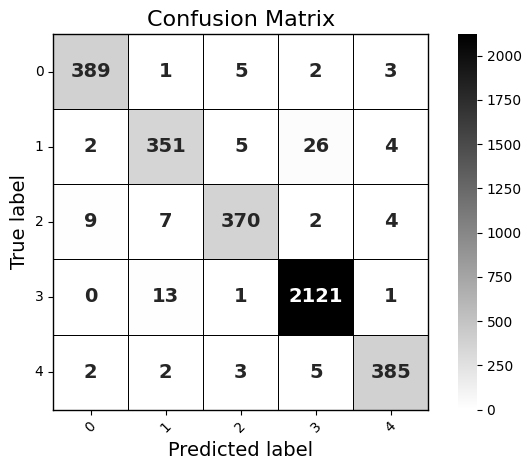
\includegraphics[width=0.7\textwidth]{Images/BAG CM.png}  
    \caption{Confusion Matrix for Ensemble Model4}
    \label{lstm arch}  % Label for referencing the figure
\end{figure}

\begin{figure}[h!]  
    \centering
    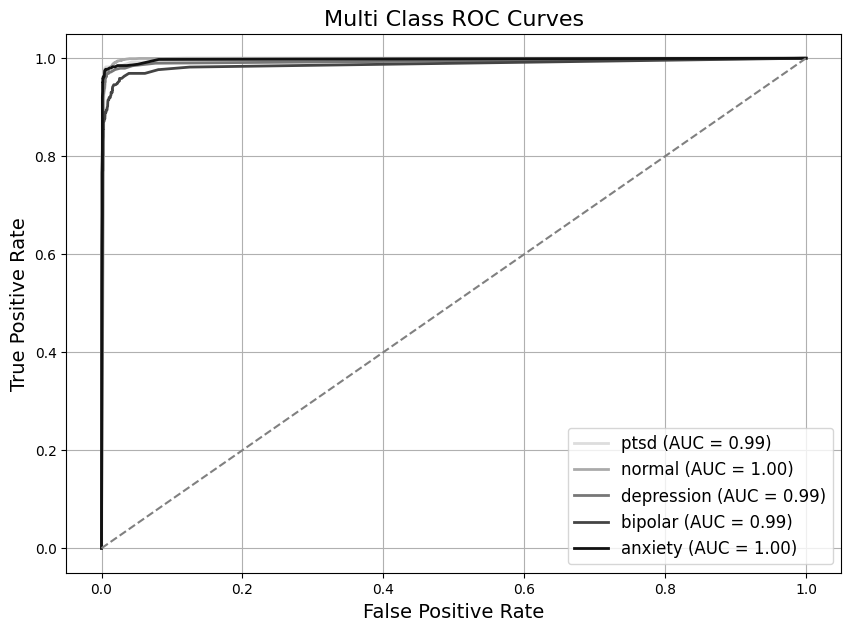
\includegraphics[width=0.7\textwidth]{Images/BAG ROC.png}  
    \caption{ROC AUC for Ensemble Model4}
    \label{lstm arch}  % Label for referencing the figure
\end{figure}

\begin{figure}[h!]  
    \centering
    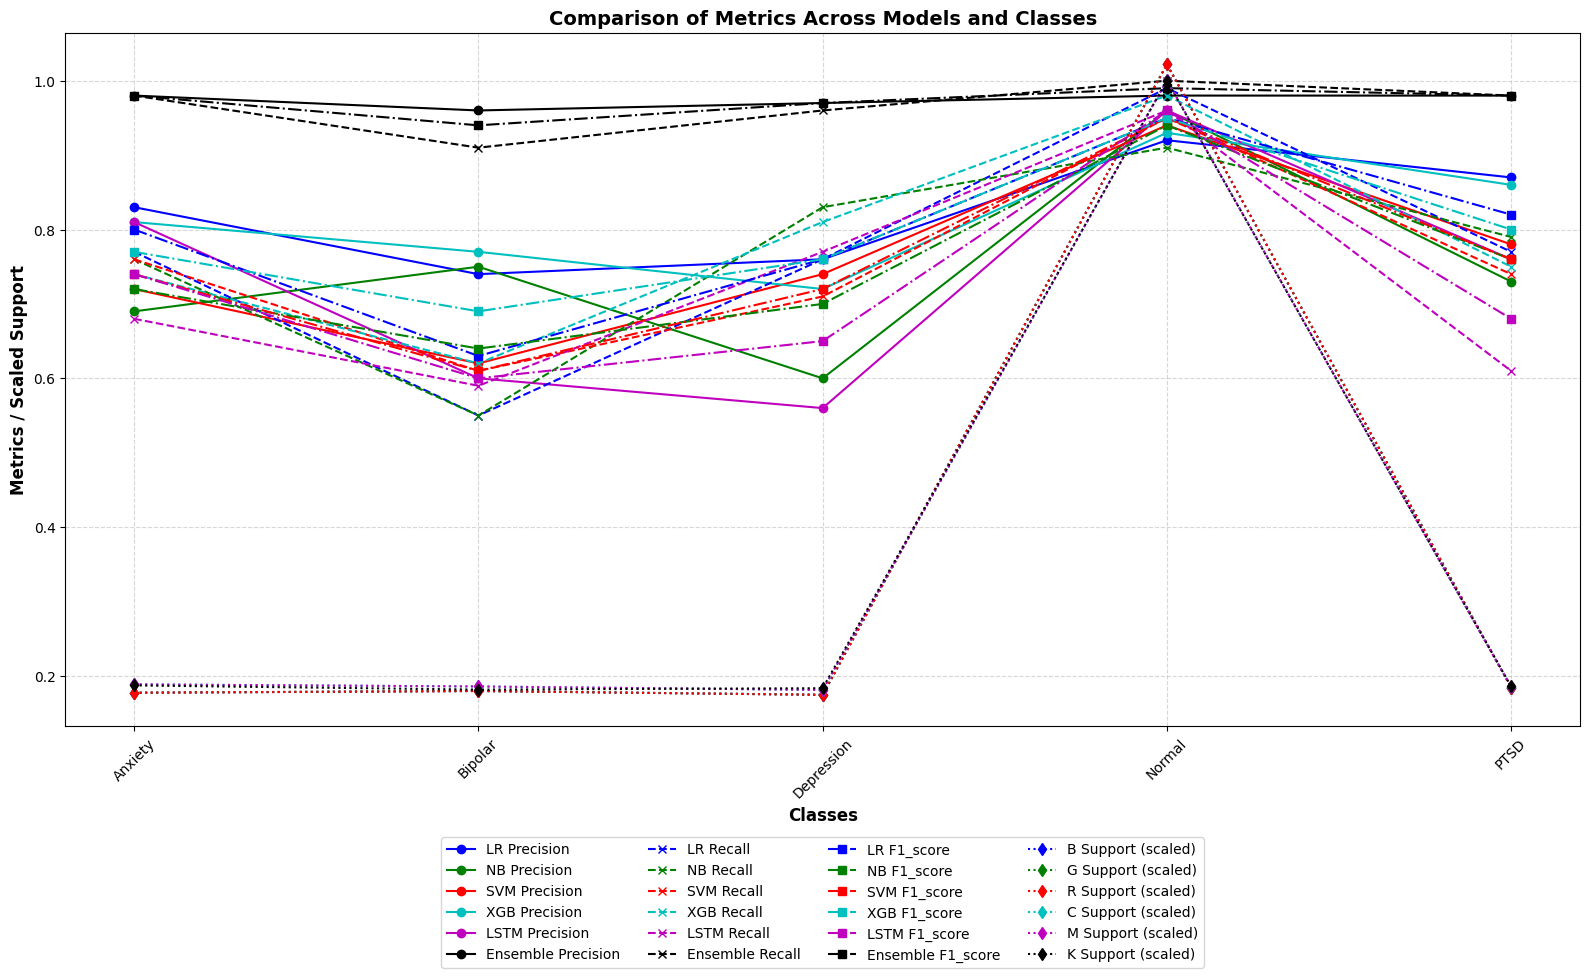
\includegraphics[width=1.0\textwidth]{Images/BAG RESULT.png}  
    \caption{Comparison of Base Models and Ensemble Model4}
    \label{lstm arch}  % Label for referencing the figure
\end{figure}

\noindent
The classification results for the Bagging model demonstrate high performance, with an accuracy of 97.63\%. The classification report highlights strong precision, recall, and F1-scores across all classes, confirming the model's capability to accurately identify and classify mental health states. Notably, the "Normal" class exhibits near-perfect classification with precision, recall, and F1-scores all close to 0.99. Other classes, such as "Anxiety," "Bipolar," and "PTSD," also maintain high performance with minimal errors. The confusion matrix reveals minimal misclassifications. For example, in the "Anxiety" class, only a small number of instances are misclassified into other categories, while the "Bipolar" class shows a slightly higher degree of misclassification but still achieves a recall of 0.90 and an F1-score of 0.92. These results emphasize the robustness of the Random Forest model in handling complex datasets.

\noindent
Bagging classifiers, while highly effective at improving predictive accuracy, have a tendency to overfit the training data when used as meta-learners in ensemble models. This is due to the way bagging works, which involves training multiple base models on bootstrapped subsets of the training data and averaging their predictions. Although this method reduces variance in individual models, it can inadvertently lead to overfitting. Bagging classifiers aggregate outputs from high-variance base models, and when used as a meta-learner, the bagging process leverages outputs from already strong individual classifiers such as SVM, XGBoost, and LSTM. This additional layer of aggregation may amplify the model's capacity to memorize the training data, particularly when the meta-learner is exposed to intricate patterns that are not generalizable to unseen data. This can result in high accuracy on the training set but poor generalization to new data. The Bagging classifier can achieve an impressive accuracy, such as 99.77\%, but this performance might not hold in real-world scenarios due to its reduced ability to generalize. When the model encounters slight variations in the testing dataset, its overfitting nature can cause the model to fail in maintaining consistent accuracy, leading to unreliable predictions. Bagging classifiers also do not inherently introduce the same level of regularization that Random Forest does. Random Forest uses feature-level randomness, selecting a subset of features for splitting at each node, which helps reduce overfitting by preventing any single feature from dominating the splits. Bagging classifiers, on the other hand, utilize all available features for training, which increases the likelihood of the model fitting noise in the training data, especially in high-dimensional datasets. Moreover, Bagging classifiers can be unstable and sensitive to minor changes in input data or individual base model outputs. This instability can further reduce the reliability of the model in practical applications, where consistency in predictions is crucial. In contrast, Random Forest, despite having slightly lower accuracy than the Bagging classifier, is better suited as a meta-learner. Random Forest introduces feature-level randomness, which prevents overfitting and enables the model to generalize well to unseen data. The bias-variance tradeoff is better balanced in Random Forest, which allows it to perform consistently across different datasets. Another significant advantage of using Random Forest as a meta-learner is its ability to maintain stability when retrained with new data inputs. For example, when retraining with user inputs, the accuracy fluctuations of the Random Forest meta-learner are minimal, indicating its robustness and ensuring stable performance over time. Additionally, Random Forest classifiers are computationally more efficient than Bagging classifiers, making them a more practical choice for real-time systems, such as those in web applications.


\subsubsection{Ensemble Model 5}

\begin{center}
    \textbf{Cross-Validation Accuracy Scores} \\[0.5em]
    \begin{tabular}{|c|c|}
        \hline
        \textbf{Cross-Validation Accuracy Scores} & \textbf{Value} \\ \hline
        1 & 0.96768765 \\ \hline
        2 & 0.97273645 \\ \hline
        3 & 0.97306397 \\ \hline
        4 & 0.96801347 \\ \hline
        5 & 0.96767677 \\ \hline
        \textbf{Mean Validation Accuracy} & \textbf{96.98\%} \\ \hline
    \end{tabular}
\end{center}

\begin{center}
    \textbf{Classification Report for Ensemble Model5} \\[0.5em]
    \begin{tabular}{|c|c|c|c|c|}
        \hline
        & \textbf{Precision} & \textbf{Recall} & \textbf{F1-Score} & \textbf{Support} \\ \hline
        \textbf{Anxiety}    & 0.96 & 0.95 & 0.96 & 400 \\ \hline
        \textbf{Bipolar}    & 0.94 & 0.89 & 0.92 & 388 \\ \hline
        \textbf{Depression} & 0.96 & 0.95 & 0.95 & 392 \\ \hline
        \textbf{Normal}     & 0.98 & 0.99 & 0.99 & 2136 \\ \hline
        \textbf{PTSD}       & 0.97 & 0.97 & 0.97 & 397 \\ \hline
        \textbf{Accuracy}   & \multicolumn{4}{c|}{\textbf{97.17\%}} \\ \hline
        \textbf{Macro avg}  & 0.96 & 0.95 & 0.96 & 3713 \\ \hline
        \textbf{Weighted avg} & 0.97 & 0.97 & 0.97 & 3713 \\ \hline
    \end{tabular}
\end{center}


\begin{center}
    \textbf{ROC AUC Scores} \\[0.5em]
    \begin{tabular}{|c|c|}
        \hline
        \textbf{Class} & \textbf{AUC Score} \\ \hline
        Anxiety        & 1.00 \\ \hline
        Bipolar        & 0.99 \\ \hline
        Depression     & 1.00 \\ \hline
        Normal         & 1.00 \\ \hline
        PTSD           & 1.00 \\ \hline
    \end{tabular}
\end{center}

\begin{figure}[h!]  
    \centering
    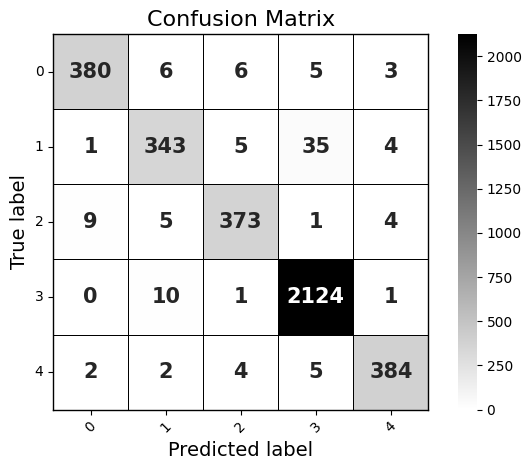
\includegraphics[width=0.7\textwidth]{Images/BLD CM.png}  
    \caption{Confusion Matric for Ensemble Model5}
    \label{lstm arch}  % Label for referencing the figure
\end{figure}

\begin{figure}[h!]  
    \centering
    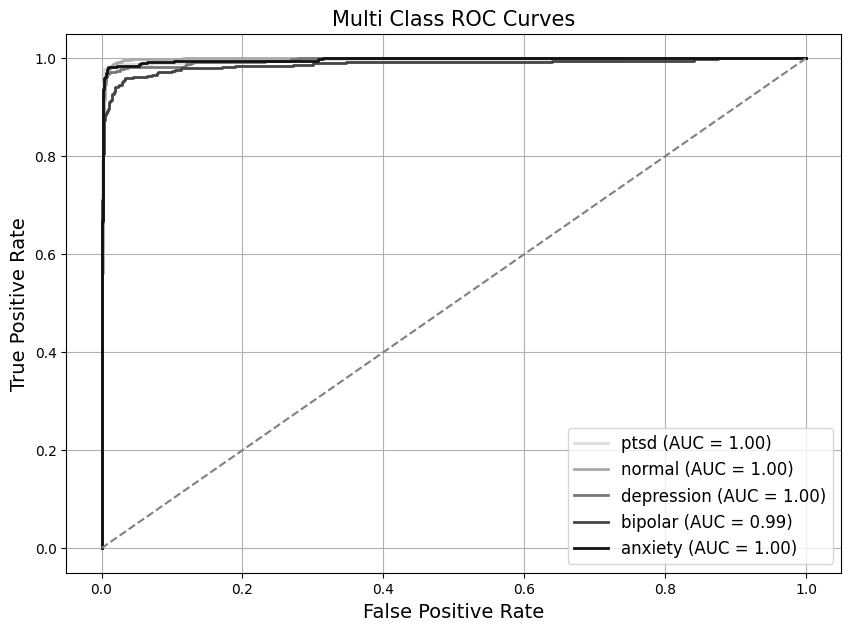
\includegraphics[width=0.7\textwidth]{Images/BLD ROC.png}  
    \caption{ROC AUC for Ensemble Model5}
    \label{lstm arch}  % Label for referencing the figure
\end{figure}

\begin{figure}[h!]  
    \centering
    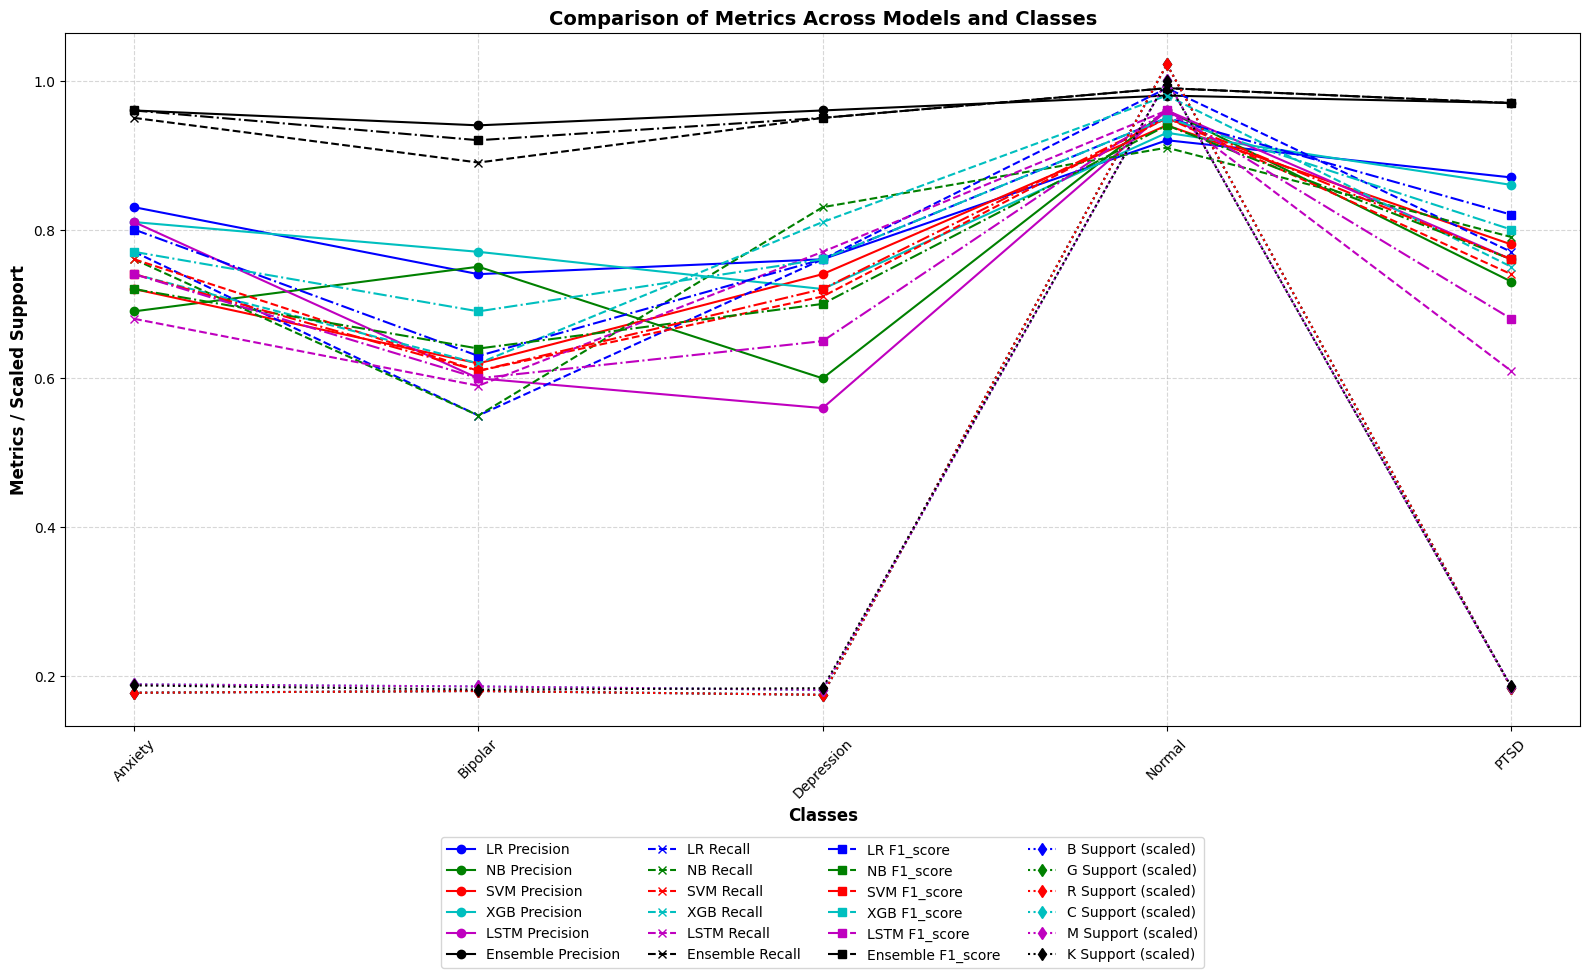
\includegraphics[width=1.0\textwidth]{Images/BLD RESULT.png}  
    \caption{Comparison of Base Models and Ensemble Model5}
    \label{lstm arch}  % Label for referencing the figure
\end{figure}

\noindent
The Blending Meta-Learner model exhibits strong performance with a test accuracy of 97.17\%. The classification report highlights solid precision, recall, and F1-scores across all classes, confirming the model's ability to accurately classify mental health conditions. For anxiety, the precision, recall, and F1-score are 0.96, 0.95, and 0.96 respectively, indicating high accuracy in classifying anxiety. The bipolar class shows a precision of 0.94 and recall of 0.89, with an F1-score of 0.92. Depression has an excellent performance with precision, recall, and F1-score of 0.96, 0.95, and 0.95, respectively. The normal class shows near-perfect classification with precision of 0.98, recall of 0.99, and F1-score of 0.99, highlighting the model's ability to accurately predict the majority class. PTSD shows a precision of 0.97, recall of 0.97, and F1-score of 0.97, reflecting strong performance. The accuracy across all classes is 97\%, with the macro average F1-score being 0.96, and the weighted average F1-score being 0.97. The confusion matrix reveals minimal misclassifications, with anxiety, bipolar, and depression showing only a few misclassified instances, and the normal class showing very few errors. The ROC AUC scores indicate excellent model performance in distinguishing between classes, with perfect scores of 1.00 for anxiety, depression, normal, and PTSD, and a score of 0.99 for bipolar. Cross-validation results show consistency, with accuracies ranging from 96.77\% to 97.31\% and a mean validation accuracy of 96.98\%. The standard deviation of validation accuracy is 0.25\%, demonstrating the stability of the model across different folds. These results emphasize the effectiveness and reliability of the Blending Meta-Learner in predicting mental health conditions with minimal misclassifications and high consistency. However, despite these impressive results, stacking ensemble using Random Forest as the meta-learner is often preferred over this Blending model. The main reason for this is that stacking tends to be more effective in generalizing to unseen data because it leverages multiple models for training the meta-learner, which reduces the risk of overfitting. In contrast, Blending may result in overfitting as it typically uses a simpler approach of directly training the meta-learner on the predictions from base models without incorporating a cross-validation step.



\subsubsection{Ensemble Model 6}

\begin{center}
    \textbf{Cross-Validation Accuracy Scores} \\[0.5em]
    \begin{tabular}{|c|c|}
        \hline
        \textbf{Cross-Validation Accuracy Scores} & \textbf{Value} \\ \hline
        1 & 0.9582547805009426 \\ \hline
        2 & 0.9477511446269863 \\ \hline
        3 & 0.9453272286560732 \\ \hline
        4 & 0.9464045246431457 \\ \hline
        5 & 0.9488284406140587 \\ \hline
        \textbf{Mean Validation Accuracy} & \textbf{94.93\%} \\ \hline
    \end{tabular}
\end{center}

\begin{center}
    \textbf{Classification Report for Ensemble Model6} \\[0.5em]
    \begin{tabular}{|c|c|c|c|c|}
        \hline
        & \textbf{Precision} & \textbf{Recall} & \textbf{F1-Score} & \textbf{Support} \\ \hline
        \textbf{Anxiety}    & 0.95 & 0.92 & 0.94 & 400 \\ \hline
        \textbf{Bipolar}    & 0.96 & 0.74 & 0.84 & 388 \\ \hline
        \textbf{Depression} & 0.92 & 0.94 & 0.93 & 392 \\ \hline
        \textbf{Normal}     & 0.95 & 1.00 & 0.97 & 2136 \\ \hline
        \textbf{PTSD}       & 0.98 & 0.93 & 0.96 & 397 \\ \hline
        \textbf{Accuracy}   & \multicolumn{4}{c|}{\textbf{95.15\%}} \\ \hline
        \textbf{Macro avg}  & 0.95 & 0.91 & 0.93 & 3713 \\ \hline
        \textbf{Weighted avg} & 0.95 & 0.95 & 0.95 & 3713 \\ \hline
    \end{tabular}
\end{center}

\begin{center}
    \textbf{ROC AUC Scores} \\[0.5em]
    \begin{tabular}{|c|c|}
        \hline
        \textbf{Class} & \textbf{ROC AUC} \\ \hline
        Anxiety & 1.00 \\ \hline
        Bipolar & 0.99 \\ \hline
        Depression & 1.00 \\ \hline
        Normal & 1.00 \\ \hline
        PTSD & 1.00 \\ \hline
    \end{tabular}
\end{center}

\begin{figure}[h!]  
    \centering
    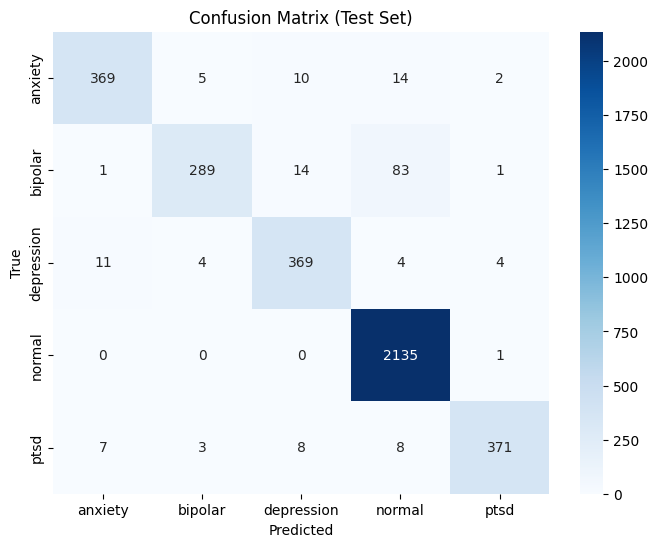
\includegraphics[width=0.7\textwidth]{Images/WV CM.png}  
    \caption{Confusion Matrix for Ensemble Model6}
    \label{lstm arch}  % Label for referencing the figure
\end{figure}

\begin{figure}[h!]  
    \centering
    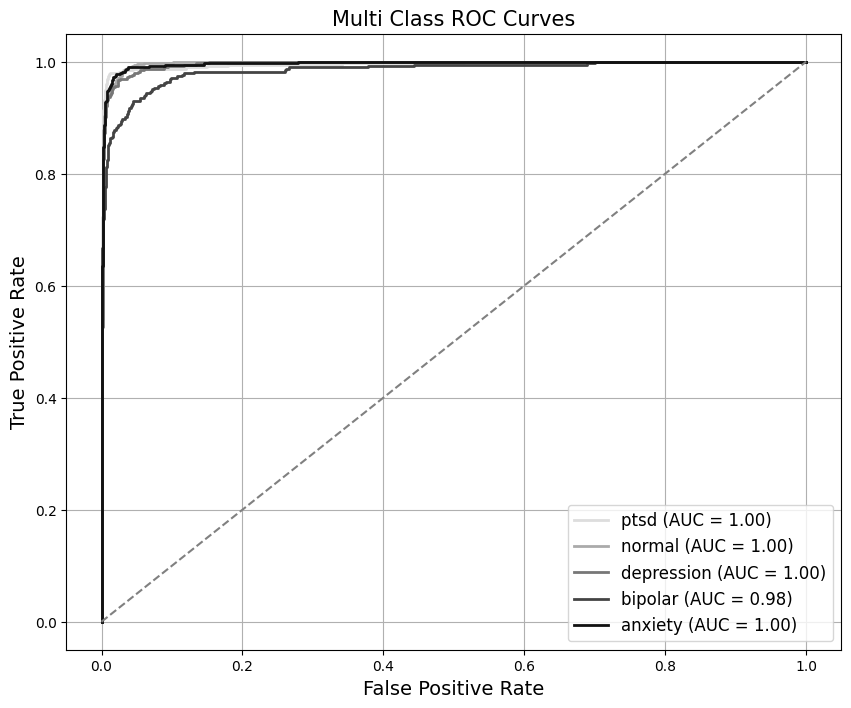
\includegraphics[width=0.7\textwidth]{Images/WV ROC.png}  
    \caption{ROC for Ensemble Model6}
    \label{lstm arch}  % Label for referencing the figure
\end{figure}

\begin{figure}[h!]  
    \centering
    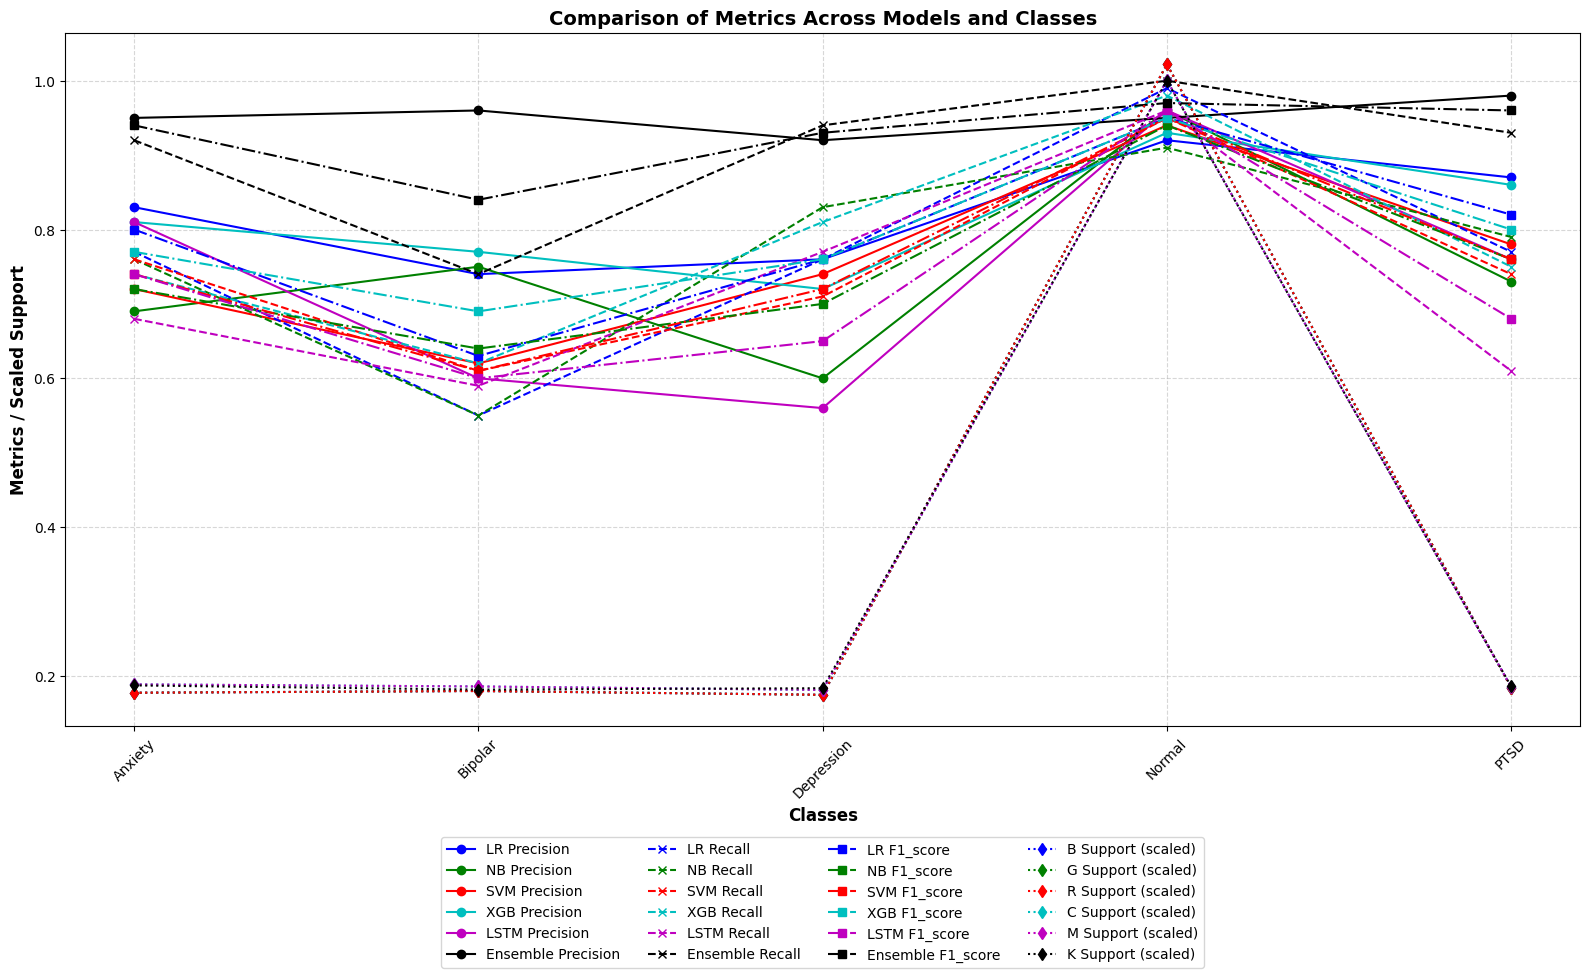
\includegraphics[width=1.00\textwidth]{Images/WV RESULT.png}  
    \caption{Comparison of Base Models and Ensemble Model6}
    \label{lstm arch}  % Label for referencing the figure
\end{figure}

\noindent
The Weighted Voting model achieved an accuracy of 95.15\% on the test set, showcasing solid performance across multiple mental health categories. The classification report reveals that the model performed particularly well in identifying "Normal" cases, with perfect recall (1.00) and high precision (0.95). While the "Bipolar" class showed the lowest recall (0.74) and precision (0.96), indicating some challenges in correctly identifying bipolar disorder, other classes like "Anxiety" and "PTSD" exhibited strong performance with high F1-scores (0.94 and 0.96, respectively). The confusion matrix further highlights a few misclassifications, with a notable number of "Bipolar" instances misclassified as other classes, particularly "Normal" and "Depression." The ROC AUC score of 0.99 for PTSD indicates that the model performed exceptionally well in distinguishing PTSD cases from the rest, though other classes had lower AUC values. Overall, the Weighted Voting model effectively handled the classification task with robust performance for most classes, but some room for improvement remains in distinguishing between certain mental health issues, particularly bipolar disorder.

\noindent
While the Weighted Voting ensemble model shows a respectable accuracy of 94.93\% and performs well across all classes, it is not preferred over other models like the Stacking ensemble with Random Forest as the meta-learner. The primary reason for this is that the Weighted Voting model does not fully take advantage of the strength of individual base models in the same way as the Stacking ensemble does. In Weighted Voting, the predictions of base models are combined based on their weighted contribution, but this method does not allow for the optimal learning of inter-model relationships that Stacking does. In the Stacking model, the Random Forest meta-learner is specifically designed to handle interactions between different base models, learning how to combine their strengths in a way that minimizes overfitting while maintaining high accuracy. In contrast, Weighted Voting simply assigns a weight to each model based on its performance, without a deeper mechanism to adjust for overfitting or to learn from the diversity of base models. This lack of fine-tuning in model interaction limits its ability to generalize as effectively as Stacking. Furthermore, the Weighted Voting model's performance may suffer when dealing with more complex relationships between features, as it relies on the simplicity of averaging the weighted predictions. While it is computationally efficient, it does not provide the robustness that Stacking offers through a more sophisticated meta-learning approach. As a result, despite the relatively high accuracy, the Weighted Voting ensemble model is considered less optimal for the given task when compared to more powerful models like Stacking.


\subsubsection{Ensemble Model 7}

\begin{center}
    \textbf{Cross-Validation Accuracy Scores} \\[0.5em]
    \begin{tabular}{|c|c|}
        \hline
        \textbf{Cross-Validation Accuracy Scores} & \textbf{Value} \\ \hline
        1 & 0.980878 \\ \hline
        2 & 0.97899273 \\ \hline
        3 & 0.98410988 \\ \hline
        4 & 0.98168597 \\ \hline
        5 & 0.97764611 \\ \hline
        \textbf{Mean Validation Accuracy} & \textbf{98.03\%} \\ \hline
    \end{tabular}
\end{center}

\begin{center}
    \textbf{Classification Report for Ensemble Model7} \\[0.5em]
    \begin{tabular}{|c|c|c|c|c|}
        \hline
        & \textbf{Precision} & \textbf{Recall} & \textbf{F1-Score} & \textbf{Support} \\ \hline
        \textbf{Anxiety}    & 0.98 & 0.97 & 0.98 & 400 \\ \hline
        \textbf{Bipolar}    & 0.96 & 0.93 & 0.95 & 388 \\ \hline
        \textbf{Depression} & 0.97 & 0.97 & 0.97 & 392 \\ \hline
        \textbf{Normal}     & 0.99 & 1.00 & 0.99 & 2136 \\ \hline
        \textbf{PTSD}       & 0.98 & 0.98 & 0.98 & 397 \\ \hline
        \textbf{Accuracy}   & \multicolumn{4}{c|}{\textbf{98.20\%}} \\ \hline
        \textbf{Macro avg}  & 0.98 & 0.97 & 0.97 & 3713 \\ \hline
        \textbf{Weighted avg} & 0.98 & 0.98 & 0.98 & 3713 \\ \hline
    \end{tabular}
\end{center}

\begin{center}
    \textbf{ROC AUC Scores} \\[0.5em]
    \begin{tabular}{|c|c|}
        \hline
        \textbf{Class} & \textbf{ROC AUC Score} \\ \hline
        Anxiety & 1.00 \\ \hline
        Bipolar & 1.00 \\ \hline
        Depression & 1.00 \\ \hline
        Normal & 1.00 \\ \hline
        PTSD & 1.00 \\ \hline
    \end{tabular}
\end{center}

\begin{figure}[h!]  
    \centering
    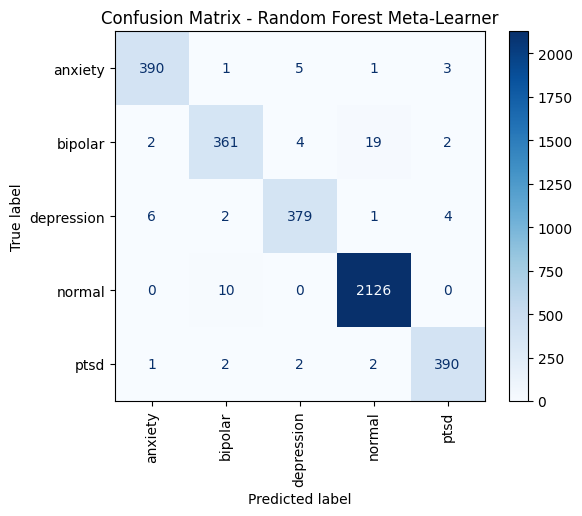
\includegraphics[width=0.7\textwidth]{Images/EM T CM.png}  
    \caption{Confusion Matrix for Ensemble Model7}
    \label{lstm arch}  % Label for referencing the figure
\end{figure}

\begin{figure}[h!]  
    \centering
    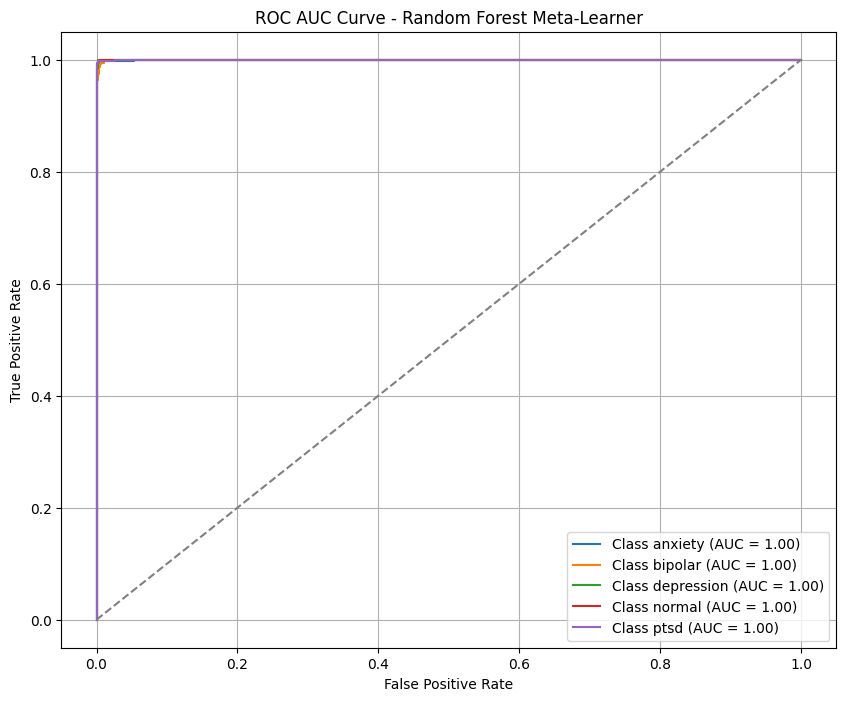
\includegraphics[width=0.7\textwidth]{Images/EM T ROC.png}  
    \caption{ROC AUC for Ensemble Model7}
    \label{lstm arch}  % Label for referencing the figure
\end{figure}

\begin{figure}[h!]  
    \centering
    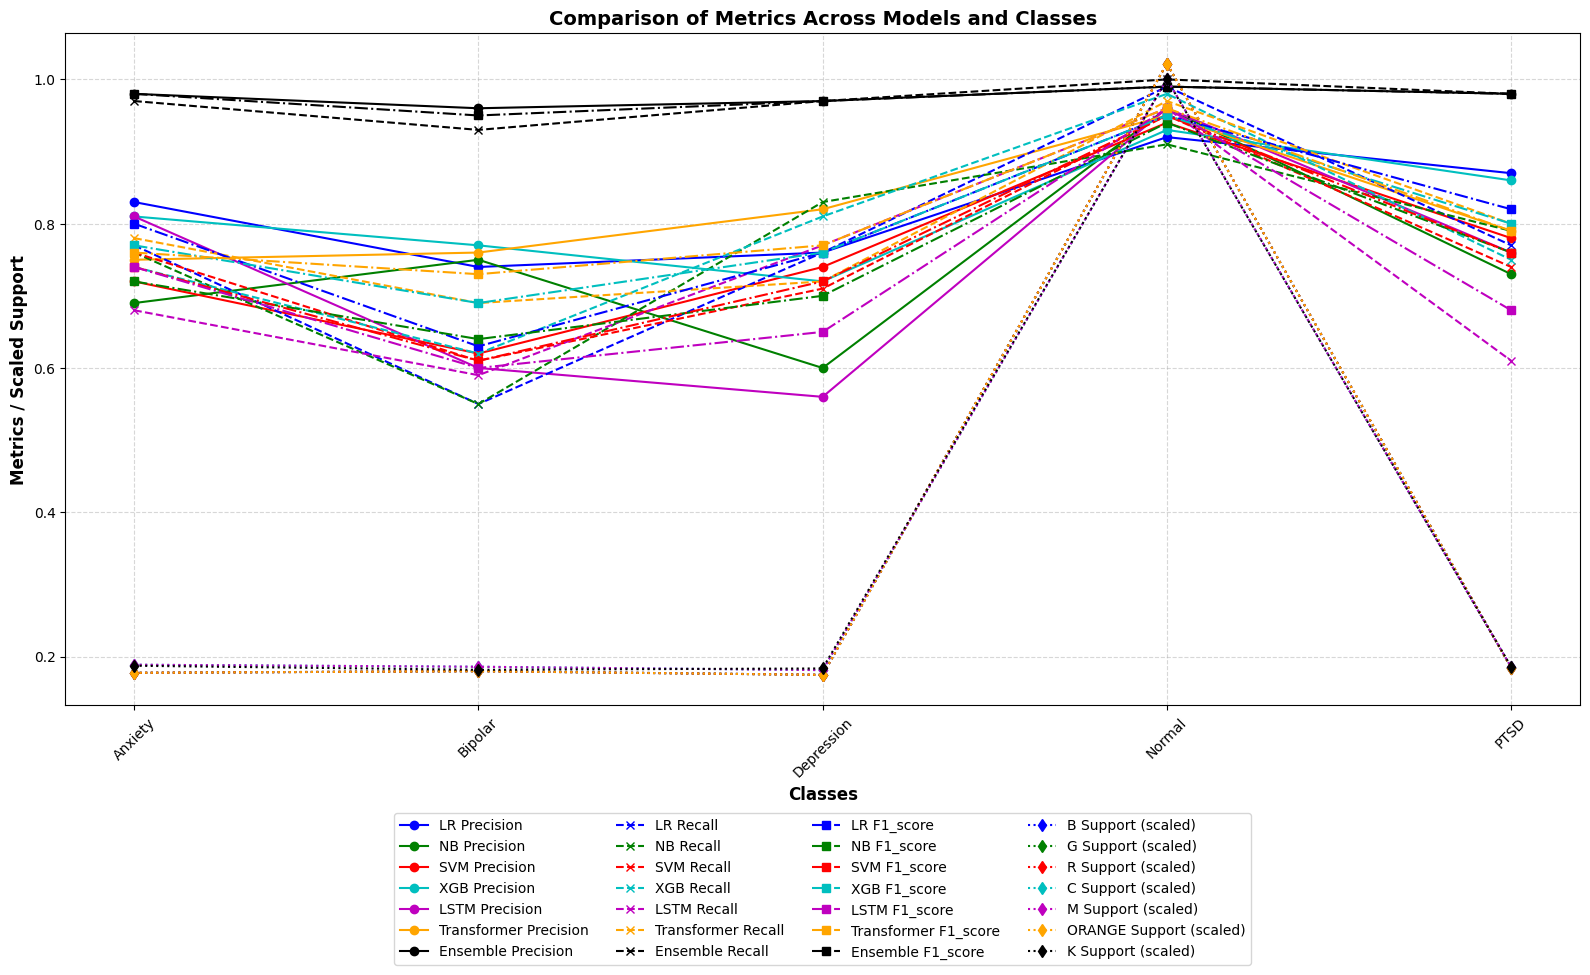
\includegraphics[width=1.0\textwidth]{Images/EM T RESULT.png}  
    \caption{Comparison of Base Models and Ensemble Model7}
    \label{lstm arch}  % Label for referencing the figure
\end{figure}

\noindent
The ensemble model, which leverages a Transformer-based model as the base learner along with Logistic Regression, Naive Bayes, SVM, LSTM, XGBoost, and Random Forest as the meta-learner, has achieved an impressive accuracy of 98.03\% on the test set. The classification report indicates high precision, recall, and F1-scores across all classes, with the model performing particularly well in detecting "Normal" and "PTSD" cases, where precision and recall are both very high. The confusion matrix reveals minimal misclassifications, further demonstrating the effectiveness of the ensemble approach in handling complex classification tasks. The perfect ROC AUC scores of 1.00 across all classes suggest that the model is able to distinguish between different mental health conditions with near-perfect specificity and sensitivity. This robust performance highlights the advantage of combining multiple models through ensemble learning, where the strengths of each model contribute to the overall improvement in classification accuracy.

\vspace{1em}

\noindent
Incorporating a custom Transformer-based model as part of the ensemble brings significant advantages in the classification task. Transformer models are particularly effective in handling sequential data due to their self-attention mechanism, which allows the model to focus on important features and long-range dependencies within the input data. This makes them particularly suited for tasks like natural language processing or time-series classification, where context plays a crucial role. By integrating a Transformer as a base model in an ensemble, the model can capture complex patterns and relationships that other models, such as Logistic Regression or Naive Bayes, may overlook. The ensemble approach benefits from the Transformer’s ability to learn sophisticated representations, while the meta-learner, in this case, Random Forest, effectively combines the outputs of various base models to enhance overall performance. This combination not only boosts accuracy but also improves the robustness and generalization capabilities of the model, making it more reliable for real-world applications. The Transformer architecture is fundamentally different from traditional models due to its self-attention mechanism, which allows the model to weigh the importance of different tokens in a sequence regardless of their distance from each other. Unlike recurrent neural networks (RNNs) or long short-term memory (LSTM) networks, which process data sequentially, Transformers are capable of processing entire sequences in parallel, which significantly speeds up training. In a Transformer, each input token is transformed into an embedding, and the self-attention mechanism computes a weighted sum of all tokens, allowing the model to capture contextual relationships between distant elements. This allows the Transformer to learn both local and global patterns effectively. For classification tasks, this ability to understand long-range dependencies in the data is crucial. For example, in text classification, words in a sentence may carry meaning only when considered in the context of other words. A Transformer can efficiently model these relationships, regardless of how far apart the words are in the input sequence. In an ensemble, the Transformer’s ability to learn complex, high-dimensional feature representations complements the more straightforward models, which may not be able to capture such intricate patterns. When used as a base model, the Transformer generates rich feature vectors, which are then processed by the meta-learner. In this case, Random Forest, a robust ensemble method, takes the output of the base models, including the Transformer, and uses it to make the final classification decision. The meta-learner helps in reducing overfitting and improving generalization by aggregating the predictions of multiple models, leading to better performance across different data distributions. By leveraging the strengths of the Transformer’s ability to understand complex relationships and the Random Forest’s ability to combine multiple models, the ensemble approach becomes highly effective in complex classification tasks.


\vspace{1em}

\noindent
Below is a comparison of all the ensemble models for reference

\begin{figure}[h!]  
    \centering
    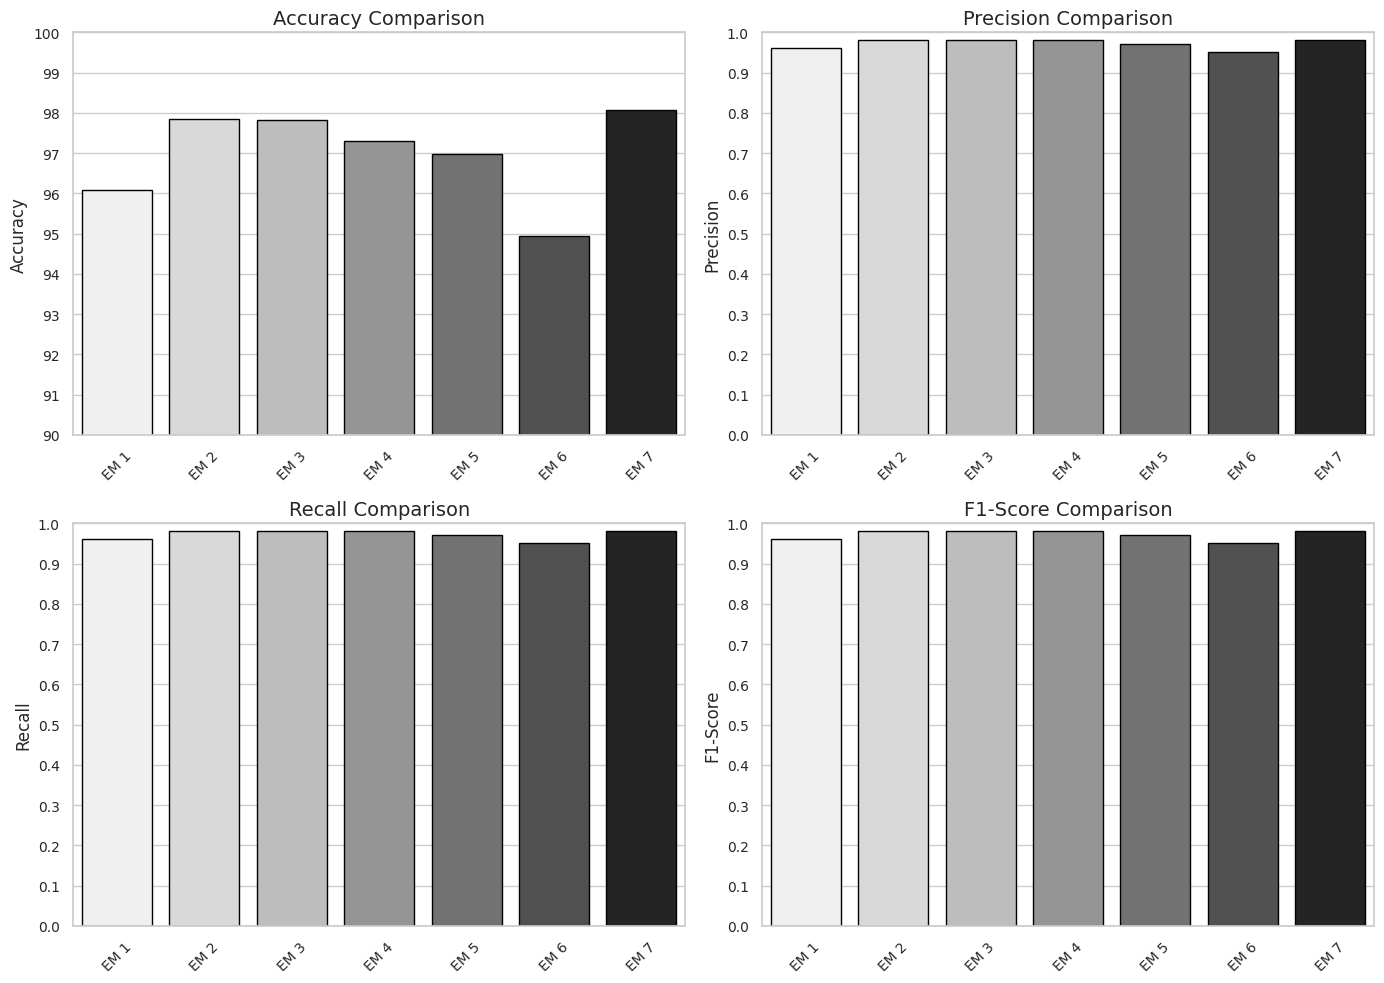
\includegraphics[width=0.77\textwidth]{Images/EM COMPARE.png}  
    \caption{Comparison of all Ensemble Models}
    \label{lstm arch}  % Label for referencing the figure
\end{figure}


\pagebreak

\subsection{Divide and Conquer}

\begin{center}
    \textbf{Performance Comparison of Models} \\[0.5em]
    \begin{tabular}{|c|c|c|c|c|c|c|}
        \hline
        \textbf{Model} & \textbf{Subset 1} & \textbf{Subset 2} & \textbf{Subset 3} & \textbf{Subset 4} & \textbf{Subset 5} & \textbf{Subset 6} \\ \hline
        Logistic Regression & 84.48 & 85.07 & 86.74 & 90.61 & 88.17 & 72.62 \\ \hline
        Naive Bayes         & 81.80 & 81.71 & 83.50 & 84.44 & 85.93 & 64.33 \\ \hline
        SVM                 & 81.45 & 82.30 & 83.50 & 88.34 & 85.45 & 67.81 \\ \hline
        XGBoost             & 84.23 & 85.79 & 86.78 & 91.37 & 86.32 & 70.95 \\ \hline
        LSTM                & 83.74 & 81.63 & 81.83 & 87.22 & 85.38 & 67.74 \\ \hline
        Transformer         & 83.21 & 84.50 & 86.50 & 89.35 & 87.62 & 72.40 \\ \hline
        \textbf{Ensemble}   & \textbf{98.20} & \textbf{97.53} & \textbf{98.02} & \textbf{96.40} & \textbf{96.15} & \textbf{91.92} \\ \hline
    \end{tabular} \\[1em]
    \textbf{Note:} The final ensemble meta-model achieved an accuracy of \textbf{96.24\%}.
\end{center}

\noindent
The hierarchical ensemble model implemented in this project addresses the challenge of handling large datasets effectively by leveraging a modular and scalable approach. The dataset, consisting of millions of records, is divided into manageable subsets, with each subset treated as an independent data unit. For each subset, multiple base models such as Logistic Regression, Naive Bayes, SVM, LSTM, XGBoost, and Custom Transformers are trained and tested. These base models are then combined into a subset-specific ensemble using Random Forest as the meta learner. This process is repeated for all subsets, resulting in several independent ensemble models. Finally, the outputs from these subset-specific ensembles are aggregated to form a final ensemble model, representing the comprehensive learning from the entire dataset. This approach not only ensures better performance but also provides a framework for handling large-scale data efficiently. While the current implementation follows a fully sequential approach for testing and validation purposes, the design is inherently scalable to a distributed system architecture. In a distributed setup, the dataset can be partitioned and processed in parallel, with each subset assigned to a separate computational node or worker. Each node trains base models, creates an ensemble for its subset, and transmits the results to a central controller. The controller aggregates the subset-specific ensembles into a global ensemble model, ensuring a streamlined process that benefits from parallelism and modularity. This architecture mirrors distributed computing principles, making it highly suitable for large-scale deployments and real-world applications. 

\vspace{1em}

\noindent
The hierarchical structure of this approach aligns with distributed systems by effectively implementing data parallelism and task parallelism. By dividing the dataset into subsets, the computational load is distributed, preventing memory bottlenecks and ensuring resource optimization. Each subset is processed independently, enabling a modular design where tasks are decoupled. This design also enhances fault tolerance, as the failure of a single subset’s processing does not affect the others. Moreover, the scalability of the approach allows it to adapt to varying resource constraints. Adding more computational nodes makes it feasible to handle additional subsets or process the data faster, showcasing its adaptability and efficiency. The project also emphasizes the potential of this design to be implemented on distributed computing frameworks such as Apache Spark, TensorFlow Distributed, or PyTorch Distributed. These frameworks provide tools to split datasets, distribute tasks, and aggregate results seamlessly across multiple nodes. The distributed nature of the architecture ensures high throughput and reduces training time, making it suitable for scenarios involving large-scale datasets. The hierarchical ensemble model design is a future-ready solution that can transition seamlessly to distributed platforms, leveraging cloud services or on-premises high-performance computing clusters. The methodology combines the strengths of ensemble learning with the efficiencies of distributed systems to create a robust and scalable solution for modern data science challenges.

\begin{figure}[h!]  
    \centering
    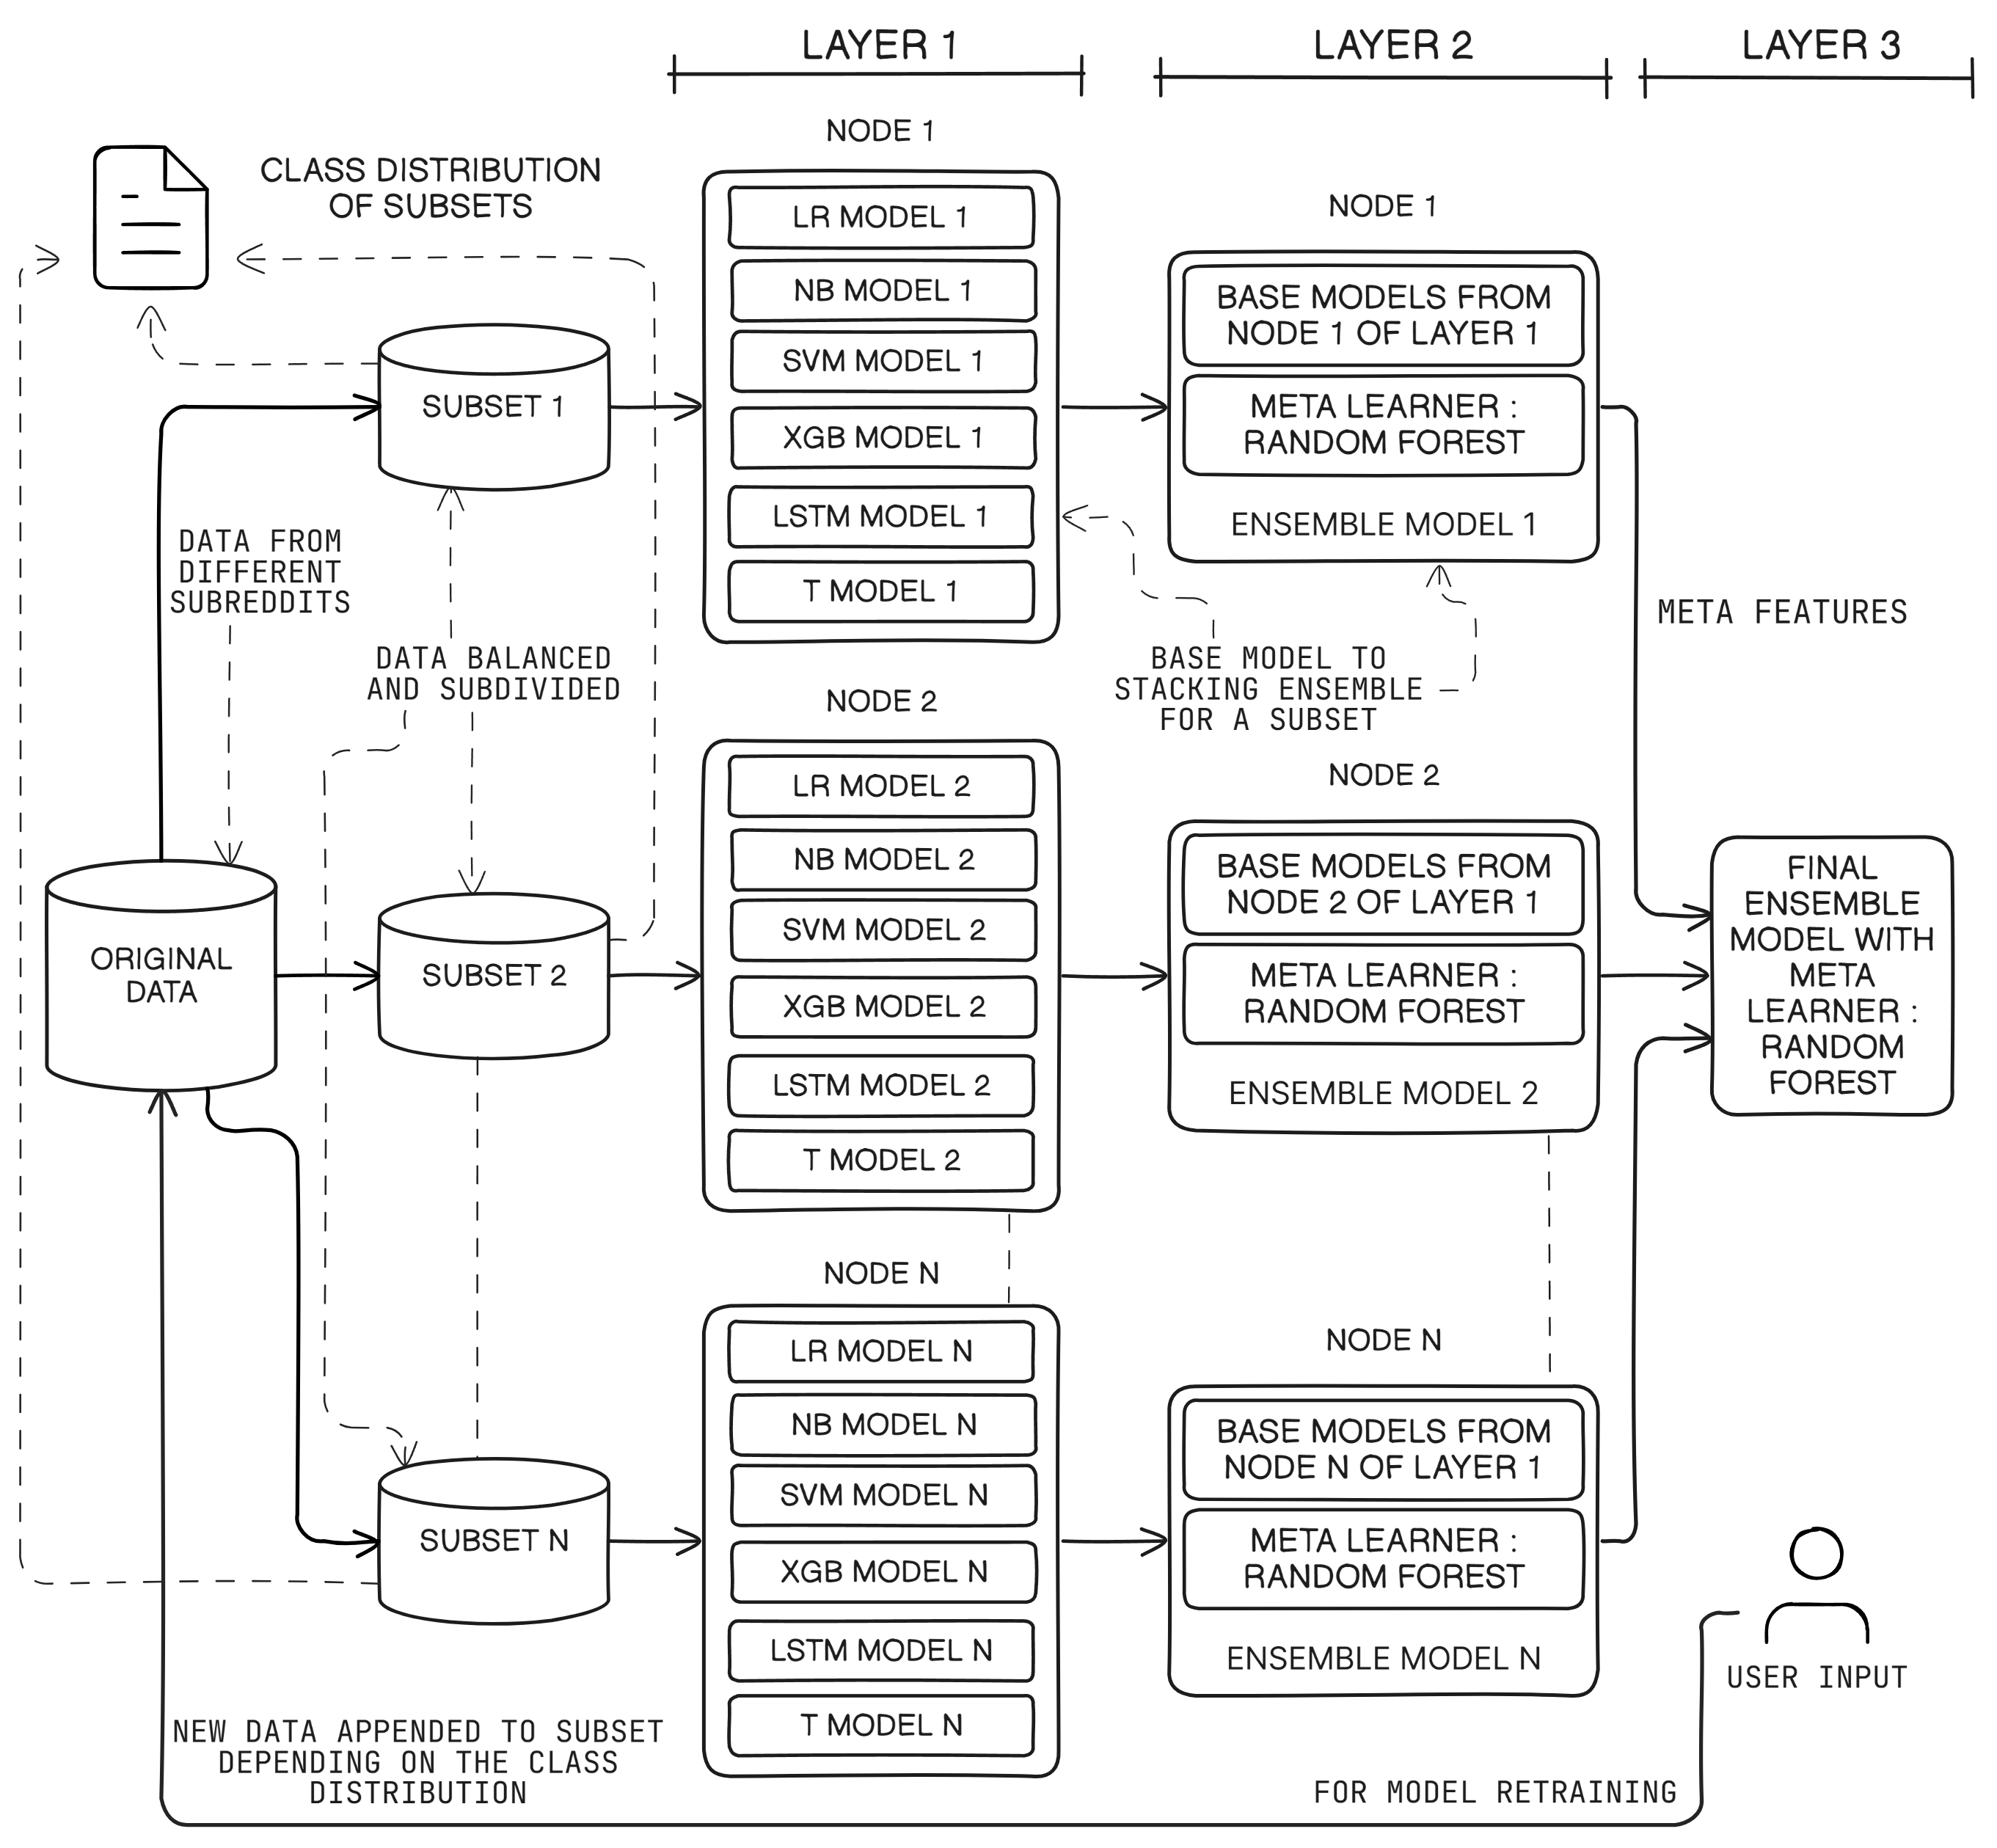
\includegraphics[width=1.0\textwidth]{Images/Distributed.png}  
    \caption{Scalable Distributed Architecture}
    \label{lstm archi}  % Label for referencing the figure
\end{figure}


\pagebreak

% ------------------------ Result and Analysis Ends -------------------------
